% ======================================================== %
% Przeczytaj plik amuthesis-doc.pdf, aby poznać opcje      %
% klasy `amuthesis`                                        %
% ======================================================== %
\documentclass[oneside,polski,logo]{amuthesis}

% Zdefiniuj kodowanie pliku źródłowego (domyślnie utf8)
\usepackage[utf8]{inputenc}
\usepackage{tikz}
% ======================================================== %
% Dane autora i pracy                                      %
% ======================================================== %

% --- Autor pracy
\author{Bohdan Bondar, Marcin Jałoński, Aleksander Mendoza-Drosik}
% --- Numer albumu
\album{sS432778,s434701,s434749}
% --- Tytuł pracy (w języku polskim i angielskim)
\titlePL{Solomonoff - kompilator transduktorów skończenie stanowych}
\titleEN{Solomonoff - Finite state tranducer compiler}
% --- Typ pracy (inżynierska, licencjacka, magisterska)
\type{inżynierska}
% --- Wydział (wykaz skrótów):
% --- --- WA    --- Wydział Anglistyki
% --- --- WB    --- Wydział Biologii
% --- --- WCh   --- Wydział Chemii
% --- --- WFPiK --- Wydział Filologii Polskiej i Klasycznej
% --- --- WF    --- Wydział Fizyki
% --- --- WH    --- Wydział Historyczny
% --- --- WMiI  --- Wydział Matematyki i Informatyki
% --- --- WNGiG --- Wydział Nauk Geograficznych i Geologicznych
% --- --- WNPiD --- Wydział Nauk Politycznych i Dziennikarstwa
% --- --- WNS   --- Wydział Nauk Społecznych
% --- --- WN    --- Wydział Neofilologii
% --- --- WPAK  --- Wydział Pedagogiczno-Artystyczny w Kaliszu
% --- --- WPiA  --- Wydział Prawa i Administracji
% --- --- WSE   --- Wydział Studiów Edukacyjnych
% --- --- WT    --- Wydział Teologiczny
% --- --- IKE   --- Instytut Kultury Europejskiej w Gnieźnie
\faculty{WMiI}
% --- Kierunek (w mianowniku)
\field{informatyka}
% --- Specjalność (w formie mianownikowej)
% --- (ustaw puste, jeśli bez specjalności)
\specialty{}
% --- Promotor (w dopełniaczu)
\supervisor{dr Bartłomieja Przybylskiego}
% --- Data złożenia pracy (Miasto, miesiąc rok)
\date{Poznań, luty 2021}

% --- Płeć autora (M/K)
\stsex{M/M/M}
% --- Zgoda na udostępnienie pracy w czytelni (TAK/NIE)
\stread{TAK/TAK/TAK}
% --- Zgoda na udostępnienie pracy w zakresie ochrony (TAK/NIE)
\stprotect{TAK/TAK/TAK}
% --- Data podpisania oświadczenia (Miasto, data)
\stdate{Poznań, \today{} r.}

% ======================================================== %
% Dodatkowe pakiety wykorzystywane w pracy                 %
% ======================================================== %

\usepackage{lipsum}

% ======================================================== %
% Zasadnicza część dokumentu                               %
% ======================================================== %

\begin{document}

% Strona tytułowa
\maketitle
% Oświadczenie
\makestatement

% Blok abstraktu w języku polskim
\begin{streszczenie}



\paragraph{Słowa kluczowe:} klasa
\end{streszczenie}

% Blok abstraktu w języku angielskim
\begin{abstract}
\lipsum[2]

\paragraph{Keywords:} klasa
\end{abstract}

% Opcjonalny blok dedykacji
\begin{dedykacja}
Tu możesz umieścić swoją dedykację.
\end{dedykacja}

% Spis treści
\tableofcontents

% ======================================================== %
% Właściwa część pracy                                     %
% ======================================================== %


\chapter{Introduction}


This project focuses on research in the field of automata theory and inductive inference.  The main product of our work is the "Solomonoff" regular expression compiler for finite state transducers. Plenty of research has gone into development of the theory behind this system. As a result the transducers contain several features not know before. 

The most innovative achievements is the lexicographic arctic semiring of weights, specialized adaptation of Glushkov's construction for subsequential transducers and the most significant flagship feature - built-in support for inductive inference and machine learning of transducers. Thanks to the cooperation with LearnLib and Dortmund University, Solomonoff supports learning algorithms such as RPNI and several of it's  derivatives. Solomonoff contributes its own more specialized for transducers inference. We implemented OSTIA for efficient learning of deterministic transducers. For nondeterministic ones we developed our own OFTIA algorithm, that was not known before. 

All those features together make Solomonoff a unique library that stands out from all the alternatives. We support most of the features of UNIX regexes, including look-aheads and look-behinds, which is unusual for automata-based regex engine. The key that allows Solomonoff for doing that is the possibility of emulating look-aheads with careful placement of transducer outputs. As a result Solomonoff can compete and  do much more than existing projects such as RE2 developed by Google, BRICKS automata developed at  Aarhus University or even to certain extent with Pearl/Java based regular expression engines. Another, much stronger competitor for Solomonoff is the OpenFST project developed by Google. Their Thrax grammars are capable of doing most of the things that Solomonoff can and they also support probabilistic automata. OpenFST is much older and more established in the scientific community. They support a lot more features that were developed by scientists, by the course of many years. Solomonoff cannot compete with this level of sophistication, but perhaps, what might seem like a limitation, is in fact our strongest advantage. Solomonoff focuses on functional transducers and enforces this property at compilation time. Any arising nondeterministic output is automatically rejected as an error. This allows Solomonoff to perform a lot more optimisations, the automata are smaller and their behaviour is more predictable. Moreover, lexicographic weights allow for precise disambiguation of nondeterministic paths whenever necessary and their most important advantage is that lexicographic semiring is not commutative and hence it does not "propagate" throughout entire automaton. This only increases Solomonoff's robustness and allows for (exponentially) smaller automata, without sacrificing predictability of the regular expression. On th contrary, probabilistic weights in Thrax, make the whole system, more heavyweight, unpredictable and difficult to maintain. The results are especially palpable when comparing our benchmarks. Solomonoff was written in Java and Thrax uses C++, but despite this our compiler is several magnitudes more efficient. We performed efficiency tests on a large corpus of linguistic data (dictionary with 6000 records). Solomonoff compilation times were around 2 seconds, whereas Thrax took 19 minutes. Solomonoffs automata were also much smaller, as thanks to Glushkov's construction, there is a 1:1 relationship between size of regular expression and size of transducer. As a result Thrax's transducer takes of 6336K of RAM, whereas Solomonoff only takes 738K. Execution time for such large corpora was about 10 miliseconds in Solomonoff (which is roughly the same performance as using Java's HashMap), while Thrax took about 250 miliseconds. One might argue that, such great differences are achievable, only because Thrax supports a lot more features. OpenFST uses epsilon transitions, while Solomonoff does not implement them and instead all automata are always and directly produced in epsilon-free form. OpenFST performs operations such as sorting of edges, determinization, epsilon-removal and minimization. Solomonoff always has all of its edges sorted and it doesn't need a special routine for it (which makes for additional performance gains), it has no epsilons to remove and it does not need determinization procedure, because it can pseudo-minimise nondeterministic transducers, using heuristics inspired by Kameda-Weiner's NFA minimization. One could, half-jokingly, summarize that the difference between Thrax and Solomonoff is like that between "Android and Apple". Thrax wants to support "all of the features at all cost", whereas Solomonoff carefully chooses the right features to support. We believe this approach will be our strongest asset, that will make our compiler a serious alternative to the older and more established OpenFST. An additional strength that favours Solomonoff over OpenFST is that we support inductive inference out-of-the-box, require no programming (regular expressions are the primary user interface and Java API is minimal and optional) and we provide automatic conversion from Thrax to Solomonoff, so that existing codebases can be easily migrated.

The characteristic feature of Solomonoff, is that its development focuses on the compiler and regular expressions instead of library API. Everything can be done without writing any Java code. It also allows the developers for much greater flexibility, because the internal implementation can be drastically changed at any time, without breaking existing regular expressions. There is very little public API that needs to be maintained. As a result backwards-compatibility is rarely an issue.  

The primary philosophy used in implementing this library is the top-down approach. Features are added conservatively in a well thought-through manner. No features will be added ad-hoc. Everything is meant to fit well together and follow some greater design strategy. For comparison, consider the difference between OpenFst and Solomonoff.

\begin{itemize}
	\item OpenFst has Matcher that was meant to compactify ranges. In Solomonoff all transitions are ranged and follow the theory of (S,k)-automata. They are well integrated with regular expressions and Glushkov's construction. They allow for more efficient squaring and subset construction. Instead of being an ad-hoc feature, they are well integrated everywhere.
	
	\item OpenFst had no built-in support for regular expression and it was added only later in form of Thrax grammars, that aren't much more than another API for calling library functions. In Solomonoff the regular expressions are the primary and only interface. Instead of having separate procedures for union, concatenation and Kleene closure, there is only one procedure that takes arbitrary regular expression and compiles it in batches. This way everything works much faster, doesn't lead to introduction of any $\epsilon$-transitions and allows for more optimisation strategies by AST manipulations. This leads to significant differences in performance.
	
\end{itemize}


While, most of other automata libraries (RE2/BRICKS) were not designed for large codebases and have no build system, Solomonoff comes with it's very own build system out-of-the-box. Thrax is the only alternative that does have a "build system" but it's very primitive and relies on generating Makefiles. Solomonoff has a well integrated tool that assembles large projects, detects cyclic dependencies, allows for parallel compilation and performs additional code optimisations. It also ships with syntax highlighting and tools that assist code refactoring. Our project strives to make automata as easy to use and accessible to mass audiences as possible. For this reason we developed a website with online playground where visitors could test Solomonoff and experiment without any setup required. The backend technology we used is Spring Boot, because it allowed for convenient integration with existing API in Java. 

While at the beginning our attempts focused on implementing the library is C, switching to Java turned out to be a major advantage. While, it's true that C allows for more manual optimisations, having a garbage collector proved to be a strong asset. The compilation relies on building automata in form of directed graphs. Each vertex itself is a separate Java object. The automaton is always kept trim because all the unreachable vertices are lost and free to be garbage collected at any time. If we tried to implement such data structure in C we would need to reinvent a simple (and most likely, less efficient) garbage collector ourselves. Manipulation of linked lists, linked graphs and other recursive data structures is not as convenient in C as it is in Java. Another advantage that Java gave us over C is that the plenty of existing infrastructure was already implemented in Java. Hence we became more compatible with Samsung's systems where Solomonoff could be deployed. We could also easily integrate our compiler with LearnLib. 

For environments where Java is not an option, Solomonoff will allow for generating automata in form of C header files that can be easily included and deployed in production code. It will not allow for manipulation of automata from C level, but our compiler was never intended to be used programmatically. There is, in fact, not much benefit from doing so. If user needs to create their custom automata manually, it's much easier to generate them in AT\&T format  and then have them read by the compiler. Later they can by manipulated with regular expressions like any other automaton. Generating AT\&T has also additional benefits, as such custom script for generating AT\&T can be attached to Solomonoff build system as an external routine and then compilation can be optimised more efficiently. An example scenario would be having two independent routines that the build system could decide to run in parallel and then it could cache the results for subsequent rebuilds. For comparison, if anybody decided to use OpenFST manually from from C++, they would need to first learn the API (which is less user friendly than learning AT\&T format) and then they would also need to implement caching and parallelization themselves. Moreover, the users are also tied to C++, whereas, AT\&T format can be generated in any language. This shows, why API for programmatic  manipulation offers little to no benefit, while imposes much more limitations. It should also be mentioned that Solomonoff allows user for implementing their own Java functions that could then be incorporated into the regular expressions as "native" calls.



\chapter{Transducers}

Solomonoff is a regular expression compiler for finite state transducers. Plenty of research has gone into development of the theory behind this system. As a result the transducers contain several features not know before. The most innovative achievements is the lexicographic arctic semiring of weights, specialized adaptation of Glushkov's construction for subsequential transducers and the most significant flagship feature - built-in support for inductive inference and machine learning of transducers. Thanks to the cooperation with LearnLib and Dortmund University, Solomonoff supports learning algorithms such as RPNI and several of it's  derivatives. Solomonoff contributes its own more specialized for transducers inference. We implemented OSTIA for efficient learning of deterministic transducers. For nondeterministic ones we developed our own OFTIA algorithm, that was not known before. All those features together make Solomonoff a unique library that stands out from all the alternatives. We support most of the features of UNIX regexes, including look-aheads and look-behinds, which is unusual for automata-based regex engine. The key that allows Solomonoff for doing that is the possibility of emulating look-aheads with careful placement of transducer outputs. As a result Solomonoff can compete and  do much more than existing projects such as RE2 developed by Google, BRICKS automata developed at  Aarhus University or even to certain extent with Pearl/Java based regular expression engines. Another, much stronger competitor for Solomonoff is the OpenFST project developed by Google. Their Thrax grammars are capable of doing most of the things that Solomonoff can and they also support probabilistic automata. OpenFST is much older and more established in the scientific community. They support a lot more features that were developed by scientists, by the course of many years. Solomonoff cannot compete with this level of sophistication, but perhaps, what might seem like a limitation, is in fact our strongest advantage. Solomonoff focuses on functional transducers and enforces this property at compilation time. Any arising nondeterministic output is automatically rejected as an error. This allows Solomonoff to perform a lot more optimisations, the automata are smaller and their behaviour is more predictable. Moreover, lexicographic weights allow for precise disambiguation of nondeterministic paths whenever necessary and their most important advantage is that lexicographic semiring is not commutative and hence it does not "propagate" throughout entire automaton. This only increases Solomonoff's robustness and allows for (exponentially) smaller automata, without sacrificing predictability of the regular expression. On th contrary, probabilistic weights in Thrax, make the whole system, more heavyweight, unpredictable and difficult to maintain. The results are especially palpable when comparing our benchmarks. Solomonoff was written in Java and Thrax uses C++, but despite this our compiler is several magnitudes more efficient. We performed efficiency tests on a large corpus of linguistic data (dictionary with 6000 records). Solomonoff compilation times were around 2 seconds, whereas Thrax took 19 minutes. Solomonoffs automata were also much smaller, as thanks to Glushkov's construction, there is a 1:1 relationship between size of regular expression and size of transducer. As a result Thrax's transducer takes of 6336K of RAM, whereas Solomonoff only takes 738K. Execution time for such large corpora was about 10 miliseconds in Solomonoff (which is roughly the same performance as using Java's HashMap), while Thrax took about 250 miliseconds. One might argue that, such great differences are achievable, only because Thrax supports a lot more features. OpenFST uses epsilon transitions, while Solomonoff does not implement them and instead all automata are always and directly produced in epsilon-free form. OpenFST performs operations such as sorting of edges, determinization, epsilon-removal and minimization. Solomonoff always has all of its edges sorted and it doesn't need a special routine for it (which makes for additional performance gains), it has no epsilons to remove and it does not need determinization procedure, because it can pseudo-minimise nondeterministic transducers, using heuristics inspired by Kameda-Weiner's NFA minimization. One could, half-jokingly, summarize that the difference between Thrax and Solomonoff is like that between "Android and Apple". Thrax wants to support "all of the features at all cost", whereas Solomonoff carefully chooses the right features to support. We believe this approach will be our strongest asset, that will make our compiler a serious alternative to the older and more established OpenFST. An additional strength that favours Solomonoff over OpenFST is that we support inductive inference out-of-the-box, require no programming (regular expressions are the primary user interface and Java API is minimal and optional) and we provide automatic conversion from Thrax to Solomonoff, so that existing codebases can be easily migrated.

\chapter{Build system}

The primary goal of this project was do develop the compiler backend. 
Initially little attention was paid to structuring larger projects composed of multiple source files and dependencies. While smaller applications can work fine with a single script of regular expressions, in the tasks on natural language processing its common to build large codebases composed of millions of linguistic rules. Being able to manage and organise them efficiently becomes a major issue. 

\section{Build system as extension of compiler}

The compiler builds automata using our special version fo Glushkov's construction, which is capable of compiling subexpressions independently of each other. The results are returned in form of singly linked graph. This format allows one to parallelise compilation and split work across multiple files. For instance user could create two files \texttt{file1.mealy} and \texttt{file2.mealy}, define some variable in the first one and then use it in the second.
\begin{lstlisting}
file1.mealy:
    var1 = 'abc'
file2.mealy:
    var2 = ('prefix' var1 'suffix')*
\end{lstlisting}
Such a feature is not native to the compiler backend itself (it only parses continuous string of input) and has been delegated to the build system as an independent application instead. 

The easiest approach to implementing build system would be by concatenating all source files into one large steam of input and then feed it into the compiler.
For instance 
\begin{lstlisting}
concatenatedFiles.mealy:
    //from file1.mealy
    var1 = 'abc'
    //from file2.mealy
    var2 = ('prefix' var1 'suffix')*
\end{lstlisting}
It could be easily done with a simple Bash script or a couple of Makefiles. Despite being very straightforward, such a solution has multiple flaws. The order of concatenation matters a lot. The compiler requires that every variable is defined before being used. Should the order get mistakenly swapped, the compilation would fail. For instance 
\begin{lstlisting}
concatenatedFiles.mealy:
    //from file2.mealy
    var2 = ('prefix' var1 'suffix')* 
    // var1 used before definition!
    //from file1.mealy
    var1 = 'abc'
\end{lstlisting}
As a result, it would be user's obligation to ensure correct order of concatenation, which might quickly become unmaintainable in large projects. Second problem stems from linear types. The compiler follows the semantics of linear logic and a variable once consumed should not be reused. An explicit copy is always necessary. Hence the order of definition and usage of all variables is even more important than in other general-purpose languages that do not have linear types. For instance this will compile
\begin{lstlisting}
X = 'a'
Y = !!X 'b'
Z = X 'c'
\end{lstlisting}
but this one will fail
\begin{lstlisting}
X = 'a'
Z = X 'c'
Y = !!X 'b'
\end{lstlisting}
Third problem is that managing dependencies and building packages would become impossible. For example we might imagine code, which includes some library 
\begin{lstlisting}
include libX
X = f  // f is defined in libX
\end{lstlisting}
If in the future a new version of the library is released, it might happen that variable X is added and suddenly our code becomes invalid because we're trying to redefine X.

Our initial thought was to introduce a special function \texttt{import!('filepath')}, which would load any variable from a precompiled binary file. Then the user would write code as follows
\begin{lstlisting}
X = import!('lib/libX/f')
\end{lstlisting}
This approach suffers from one logistic problem. If user decided to split their code into several files and then import the necessary automata at will, the build system would need to detect the correct compilation order of all files. For instance if there were two files like these
\begin{lstlisting}
file X.mealy:
    a = 'a'
file Y.mealy:
    b = import!('X/a')
\end{lstlisting}
then the build system would need to first compile \texttt{X.mealy} and produce binary file \texttt{X} and only then compilation of \texttt{Y.mealy} would become possible. The major problem appears when cyclic dependencies between files arise
\begin{lstlisting}
file X.mealy:
    X = import!('Y/Y')
file Y.mealy:
    Y = import!('X/X')
\end{lstlisting}
While it's possible to create a built tool capable of detecting such problems and notifying the user, its main disadvantage is that in some cases, there might be cyclic dependency between files, despite not introducing cyclic dependencies between automata themselves. As a result, logically valid regular expressions would be prematurely rejected by build system. For example
\begin{lstlisting}
file X.mealy:
    X1 = import!('Y/Y1')
    X2 = 'a'
file Y.mealy:
    Y1 = 'b'
    Y2 = import!('X/X2')
\end{lstlisting}
The final solution we settled for was to split compilation into three phases. First the build system scans all files (in parallel) and builds abstract syntax trees of all variable definitions. In those trees there would be references to other variables that could be defined anywhere else in the project. Then in the second phase the variables would be scanned and a dependency graph would be built. We used a specialised data structure for efficiently working with directed acyclic graphs. If at any point a cycle was introduced, the build system would throw an error. Finally in the last phase every node in the graph would be compiled in parallel. For optimal performance, multiple threads would take vertices in topological order. If there is a directed edge from vertex $v_1$ to $v_2$ (meaning that variable $v_2$ depends on $v_1$), then $v_1$ will be added to the queue before $v_2$. Threads process queue entries in the FIFO order. 

\section{Implementation}

In the first phase, the parser that scans source files has been reused from the compiler backend. More precisely, the grammar of syntax is taken from the library but the build system has its own implementation of \texttt{SolomonoffGrammarListener}. Parsing is then performed using the standard ANTLR functions
\begin{lstlisting}
SolomonoffGrammarLexer lexer =
  new SolomonoffGrammarLexer(sourceFile);
SolomonoffGrammarParser parser =
  new SolomonoffGrammarParser(new CommonTokenStream(lexer));

parser.addErrorListener(new BaseErrorListener() {
    public void syntaxError(Recognizer<?, ?> recognizer, 
            Object offendingSymbol, 
            int line,
            int charPositionInLine, 
            String msg, 
            RecognitionException e) {
         System.err.println("line " + line 
         + ":" + charPositionInLine 
         + " " + msg + " " + e);
    }
});

final SolomonoffWeightedParser listener =
  new SolomonoffWeightedParser(collector, sourceFile, compiler);
ParseTreeWalker.DEFAULT.walk(listener, parser.start());
\end{lstlisting}
The listener is responsible for building abstract syntax tree for each variable and storing all definitions. Here is a fragment of ANTLR grammar that forms the list of variable definitions 
\begin{lstlisting}
funcs :
    funcs exponential='!!'? ID '=' mealy_union  # FuncDef
    | 
;
\end{lstlisting} 
Whenever some definition is parsed, the following listener callback is invoked
\begin{lstlisting}
@Override
public void exitFuncDef(FuncDefContext funcDefContext) {
    String currentVariableID = funcDefContext.ID().getText();
    SolomonoffWeighted def = stack.pop();
    collector.define(currentVariable, def);
}
\end{lstlisting}
The integral part of listener is the \texttt{collector} object. It is responsible for storing all defined variables and remembering their respective abstract syntax trees. Initially, it was enough to store a \texttt{HashMap} within the \texttt{SolomonoffWeightedParser} object and register variables using 
\begin{lstlisting}
HashMap<String,SolomonoffWeighted> idToAST = 
    new HashMap<>();
    
@Override
public void exitFuncDef(FuncDefContext funcDefContext) {
    String currentVariableID = funcDefContext.ID().getText();
    SolomonoffWeighted def = stack.pop();
    idToAST.put(currentVariable, def);
}
\end{lstlisting}
Later it was changed to a more complicated implementation, which is
\begin{lstlisting}
ConcurrentHashMap<String,SolomonoffWeighted> idToAST;
SolomonoffWeightedParser(
    ConcurrentHashMap<String,SolomonoffWeighted> shared){
    this.idToAST = shared;
}
@Override
public void exitFuncDef(FuncDefContext funcDefContext) {
    String currentVariableID = funcDefContext.ID().getText();
    SolomonoffWeighted def = stack.pop();
    idToAST.put(currentVariable, def);
}
\end{lstlisting}
In such a way, it became possible to create multiple instances of 
\texttt{SolomonoffWeightedParser} and run all of them in parallel, while the results of parsing could still be collected into one joint map.
The use of \texttt{ConcurrentHashMap} instead of regular \texttt{HashMap} allows for concurrent insertions, without requiring any locks or synchronization. 

The abstract syntax tree closely follows the definition of Solomonoff's syntax. Its formal grammar is fairly simple and mimics the mathematical definition of regular expressions
\begin{lstlisting}
mealy_union
:
    (mealy_concat bar='|') * mealy_concat # MealyUnion
;

mealy_concat
:
    mealy_concat mealy_Kleene_closure
    | mealy_Kleene_closure # MealyEndConcat
;

mealy_Kleene_closure
:
    mealy_prod  (star='*' | plus='+' | optional='?') 
    | mealy_prod # MealyNoKleeneClosure
;

mealy_prod
:
    mealy_atomic colon=':' StringLiteral # MealyProduct
    | mealy_atomic colon=':' Codepoint # MealyProductCodepoints
    | mealy_atomic # MealyEpsilonProduct
;

mealy_atomic
:
    StringLiteral # MealyAtomicLiteral
    | Range # MealyAtomicRange
    | '(' mealy_union ')' # MealyAtomicNested
;
\end{lstlisting}
In more mathematical terms it could be rewritten as
\begin{lstlisting}
regex ::= 
    regex | regex // union
    regex regex // concatenation
    regex* // Kleene closure
    : regex // output/product
    STRING_LITERAL 
    ( regex ) 
\end{lstlisting}
When presented in such a form, the algebraic data types become apparent.
A regular expression is either one of those 6 cases. Hence the above grammar could be represented as Haskell-style algebraic data type
\begin{lstlisting}
type Regex = 
    Union Regex Regex 
    | Concat Regex Regex
    | Kleene Regex
    | Output Regex
    | Brackets Regex
    | String
\end{lstlisting}
Every class in Java works like an algebraic product of its member fields. For instance the class 
\begin{lstlisting}
class X{
    A a;
    B b;
}
\end{lstlisting}
is a Cartesian product of classes $A$ and $B$. Mathematically $X=A\times B$. If $a$ is an instance of $A$ (in other words $a\in A$) and $b$ is an instance of $B$ (mathematically $b\in B$) then the pair $(a,b)$ could become an instance of $X$ (written $(a,b)\in X$). In fact, the notation for constructor $new X(a,b)$ has been inspired by mathematics. Here  $X$ is a function that returns memeber of set $X$ ($X:A \times B \rightarrow X$) and the pair $(a,b)$ is applied to $X$. The brackets $()$ should not be interpreted as syntax for function call but rather as syntax for pairs and tuples. 

Every interface is the algebraic sum of its implementations. For instance in the snippet below
\begin{lstlisting}
interface X{}
class XA{
    A a;
}
class XB{
    B b;
}
\end{lstlisting}
the type $X$ is a sum of $A$ and $B$ (written as $X=A \cup B$). The classes $XA$ and $XB$ are nothing more than projection functions. Any instance of $a\in A$ can be applied to $XA(a)$ in order to produce instance of $a\in X$. Similarly for $b\in B$ and $XB(b)\in X$.

As a result the previous Haskell code could be directly translated into Java as
\begin{lstlisting}
interface Regex{}
class Union implements Regex{
    Regex a; 
    Regex b;
}
class Concat implements Regex{
    Regex a;
    Regex b;
}
class Kleene implements Regex{
    Regex a;
}
class Output implements Regex{
    Regex a;
}
class String implements Regex{
}
\end{lstlisting}
While the standard mathematical definition of regular expressions has no place
for variables, Solomonoff does indeed extend the language of expressions with variable names. As a result we obtain one more class
\begin{lstlisting}
class Variable implements Regex{
    java.lang.String identifier;
}
\end{lstlisting}
Another deviation from mathematical definition appears when it comes to braces. It should be pointed out that they do not serve any semantic purpose. They are merely a syntactic construct. In particular, if we used reverse Polish notation, then the brackets would be unnecessary. For instance
\[
((\mbox{'a'}|\mbox{'b'}) \mbox{'c'} )*
\] 
would become
\[
* \cdot | \mbox{'a'} \mbox{'b'} \mbox{'c'}
\] 
where $\cdot$  is an explicit notation of concatenation.
The existence of braces is only required by the parser but the abstract syntax tree could function without them. In a sense, every node of the tree works like brackets by itself. Hence we do not need
\begin{lstlisting}
class Brackets implements Regex{
    Regex a;
}
\end{lstlisting}
Lastly, a few notes should be made about the \texttt{String} class.
One of the weak points of Java
 is that it artificially enforces 
 rigid hierarchy of interfaces,
 even thought it would often be
 perfectly reasonable to
 add more interfaces
 for already existing classes, such as
 java.lang.String. 
 Duck typing is a much more powerful and
 mathematically inspired paradigm, than object oriented programming.
 Thankfully, the typeclass pattern can be used to circumvent this issue.
 We can wrap any existing type in a new class and then implement any
 interface of our choice.
 \begin{lstlisting}
 class String implements Regex{
     java.lang.String str;
 }
 \end{lstlisting}
It works almost like the \texttt{impl} keyword from Rust
 \begin{lstlisting}
impl Regex for String{...}
\end{lstlisting}
The only downside of the typeclass pattern in Java is the inconvenience of overly verbose notation. It forces us to later wrap every 
\texttt{java.lang.String} in our own class, before being able to use it like an instance of \texttt{Regex}.

The abstract syntax tree is a recursive data structure and any algorithm that manipulates them must be inductive. One of the most important  algorithms is the compilation procedure. It mainly uses functions provided by compiler backend, hence it's exact implementation might look uninteresting. 
\begin{lstlisting}
interface Regex{
    G compile();
}
class Union implements Regex{
    Regex a; 
    Regex b;
    G compile(){
        return specs.union(a.compile(),b.compile());
    }
}

... the rest is done analogically...

class String implements Regex{
    java.lang.String str;
    G compile(){
        return specs.fromStr(str);
    }
}
\end{lstlisting}
The \texttt{G} class stands for singly-linked graph that encodes structure of the transducer. The above procedure strictly follows Glushkov's construction.
The exact details are implemented by \texttt{specs}, which holds reference to the compiler backend. 

To sum up, in the first phase, build system reads all source files and collects abstract syntax trees for every definition. The files are parsed in parallel. A pool of threads needs to be initialised and a queue of pending tasks is formed. This could be represented using the following code.
\begin{lstlisting}
ExecutorService pool = Executors.newWorkStealingPool();
Queue<Future<Void>> queue = new LinkedList<>();
ConcurrentHashMap<String, SolomonoffWeighted> shared = 
    new ConcurrentHashMap<>();
for (final File sourceFile : sourceFiles) {
    queue.add(pool.submit(() -> {
        SolomonoffGrammarLexer lexer =
            new SolomonoffGrammarLexer(sourceFile);
        SolomonoffGrammarParser parser =
            new SolomonoffGrammarParser(new CommonTokenStream(lexer));
        
        parser.addErrorListener(new BaseErrorListener() {...});
        
        final SolomonoffWeightedParser listener =
            new SolomonoffWeightedParser(shared);
        ParseTreeWalker.DEFAULT.walk(listener, parser.start());
        return null;
    }
}
\end{lstlisting}
In the next phase, the build system creates a dependency graph. This requires having access to all variables and their syntax trees. Hence it's necessary to wait for the parsing to complete.
\begin{lstlisting}
for (Future<Void> task : queue) {
    task.get(); // blocks until finished
}
\end{lstlisting}
In the dependency graph, every vertex represents an individual variable with
unique identifier. A dependency between two variables is formed when one variable appears in the syntax tree in the definition of another.
For instance in the following code
\begin{lstlisting}
x = 'a' | 'b'
y = 'a' (x 'b')*
\end{lstlisting}
there are two variables \texttt{x} and \texttt{y}, where \texttt{y} depends on \texttt{x}. This would translate to dependency graph on two vertices with one edge
\begin{center}
     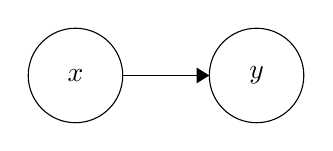
\begin{tikzpicture}[scale=0.2]
          \tikzstyle{every node}+=[inner sep=0pt]
          \draw [black] (16.5,-23.2) circle (3);
          \draw (16.5,-23.2) node {$x$};
          \draw [black] (28,-23.2) circle (3);
          \draw (28,-23.2) node {$y$};
          \draw [black] (19.5,-23.2) -- (25,-23.2);
          \fill [black] (25,-23.2) -- (24.2,-22.7) -- (24.2,-23.7);
     \end{tikzpicture}
\end{center}
The simplest way to build such a graph would be to scan every syntax tree searching for variables and then add edges accordingly. The inductive procedure could be implemented as follows
\begin{lstlisting}
interface Regex{
    void forEachVariable(Consumer<Variable> callback);
}
class Union implements Regex{
    Regex a; 
    Regex b;
    void forEachVariable(Consumer<Variable> callback){
        a.forEachVariable(callback);
        b.forEachVariable(callback);
    }
}

... the rest is done analogically...

class Variable implements Regex{
    void forEachVariable(Consumer<Variable> callback){
         callback.accept(this);
    }
}

class String implements Regex{
    java.lang.String str;
    void forEachVariable(Consumer<Variable> callback){
    }
}
\end{lstlisting}
The dependency graph is implemented using JGraphT library. It comes with a specialised data structure for directed acyclic graphs that guarantees acyclicity and throws exception whenever a newly added edge violates this property.
\begin{lstlisting}
DirectedAcyclicGraph<String, Object> dependencyOf =
    new DirectedAcyclicGraph<>(null, null, false);
\end{lstlisting}
The graph can be built by iterating all the definitions stored in \texttt{shared} map.
\begin{lstlisting}
for (Map.Entry<String, SolomonoffWeighted> def : shared.entrySet()) {
    String identifier = def.getKey();
    SolomonoffWeighted syntaxTree = def.getValue();
    syntaxTree.forEachVariable(var->{
        dependencyOf.add(
            var.identifier, // source vertex
            identifier, // target vertex
            new Object() // unique edge
        );
    });
}
\end{lstlisting}
The above code is simple but it requires to first build the syntax tree and then scan it. As a result every node of the tree is visited twice - first time during creation and second time during scanning. It also requires using the 
\texttt{forEachVariable} function. It's possible to make this procedure even simper and more efficient. The dependencies could be collected on the spot as the parsing progresses. Because multiple files are parsed in parallel
and \texttt{DirectedAcyclicGraph} is not thread-safe, an intermediate temporary storage for edges was necessary. We could first collect all of the edges into a list of pairs.
\begin{lstlisting}
List<Pair<String,String>> dependsOn;
\end{lstlisting}     
The problem with such approach is that certain edges might be duplicated. For instance consider the regular expression that uses $x$ twice
\begin{lstlisting}
x = 'a' | 'b'
y = 'a' (x 'b' x)*
\end{lstlisting}
This would lead to adding edge \texttt{Pair.of("y","x")} twice into \texttt{dependsOn}. To prevent this we use a set instead of list. The constructor of parser listener takes the following form
\begin{lstlisting}
Set<Pair<String,String>> dependsOn;
ConcurrentHashMap<String,SolomonoffWeighted> idToAST;
Set<Pair<String,String>> dependsOn;
SolomonoffWeightedParser(
         ConcurrentHashMap<String,SolomonoffWeighted> shared,
         Set<Pair<String,String>> dependsOn){
    this.idToAST = shared;
    this.dependsOn = dependsOn;
}
\end{lstlisting}
The set can be made thread-safe by using the concurrent implementation from Java standard library.
\begin{lstlisting}
ConcurrentHashMap.newKeySet()
\end{lstlisting}
The parser listener is a state-based device. When a certain rule of the formal grammar is fully parsed, several of the listener's callbacks are fired. For instance when the following rule \texttt{FuncDef} is recognized
\begin{lstlisting}
funcs :
    funcs exponential='!!'? ID '=' mealy_union  # FuncDef
    | 
;
\end{lstlisting} 
it will first fire \texttt{enterFuncDef}, then all the events hiding under \texttt{mealy\_union} are recursively executed and at the very end comes the \texttt{exitFuncDef}. If the expression contained a reference to some variable identifier at any point, then the event \texttt{exitMealyAtomicVarID} will be fired at some point during evaluation of \texttt{mealy\_union} callbacks. As a result the following code can be used to collect all dependencies into a set of pairs.
\begin{lstlisting}
String currentVariable;

@Override
public void enterFuncDef(FuncDefContext funcDefContext) {
    currentVariable = funcDefContext.ID().getText();
}
@Override
public void exitFuncDef(FuncDefContext funcDefContext) {
    SolomonoffWeighted def = stack.pop();
    idToAST.put(currentVariable, def);
}
@Override
public void exitMealyAtomicVarID(MealyAtomicVarIDContext ctx) {
    final String id = ctx.ID().getText();
    dependsOn.add(Pair.of(currentVariable,id));
    stack.push(new Variable(id));
}
\end{lstlisting}
When the parsing finishes, all of the collected dependencies need to be converted into edges of a directed graph:
\begin{lstlisting}
for (Pair<String, String> dependency : dependsOn) {
    dependencyOf.addEdge(
        dependency.right(), 
        dependency.left(), 
        new Object()
    );
}
\end{lstlisting}
If at any point a cyclic dependency is detected, the method \texttt{addEdge} will throw an exception and build system will exit prematurely.
This concludes the second phase of build procedure. 

The third and last phase is to compile all syntax trees is the correct order and parallelise it as much as possible. The compilation procedure presented before was a minimal prototype that could work with a single variable-free syntax tree.
The challenge appears when we wish to compile multiple trees that reference each other through use of variables. The simplest and most naive solution would be to substitute the variables for their appropriate referenced trees.
Such substitution could be achieved as follows
\begin{lstlisting}
interface Regex{
     Regex substitute(HashMap<String,Regex> substitution);
}
class Union implements Regex{
     Regex a; 
     Regex b;
     Regex substitute(HashMap<String,Regex> substitution){
          return new Union(
              a.substitute(substitution),
              b.substitute(substitution)
          );
     }
}

... the rest is done analogically...

class Variable implements Regex{
     String identifier;
     Regex substitute(HashMap<String,Regex> substitution){
          return substitution.get(identifier);
     }
}

class String implements Regex{
     java.lang.String str;
     Regex substitute(HashMap<String,Regex> substitution){
          return this;
     }
}
\end{lstlisting}
 As a result all syntax trees would become variable-free. This comes at the cost of possibly exponential blow-up in size of certain trees. For example consider the expression
 \begin{lstlisting}
f1 = 'a'
f2 = !!f1 f1
f4 = !!f2 f2
f8 = !!f4 f4
f16 = !!f8 f8
f32 = !!f16 f16
 \end{lstlisting}
The automaton defined by $f32$ would accept string of exponential length 32, which requires as many states.
 The major advantage is that now all trees can be independently compiled in parallel. Despite this, the compilation might in reality get worse than if we serially compiled trees with variables. That's because the overall number of nodes to be compiled could increase exponentially and the number of truly parallel threads (the number of cores in CPU) is usually small. Hence a better approach is needed. 
 
 The right solution is to compile all trees in parallel and block on variables that have not yet been processed.
 \begin{lstlisting}
 interface Regex{
      G compile(Function<String,Regex> blockingSubstitution);
 }
 class Union implements Regex{
      Regex a; 
      Regex b;
      G compile(Function<String,Regex> blockingSubstitution){
           return specs.union(
               a.compile(blockingSubstitution),
               b.compile(blockingSubstitution)
           );
      }
 }
 
 ... the rest is done analogically...
 
 class Variable implements Regex{
      String identifier;
      G compile(Function<String,Regex> blockingSubstitution){
           return blockingSubstitution.apply(identifier);
      }
 }
 
 class String implements Regex{
      java.lang.String str;
      G compile(Function<String,Regex> blockingSubstitution){
           return specs.fromStr(str);
      }
 }
\end{lstlisting}
The \texttt{blockingSubstitution} mimics the \texttt{HashMap.get} function but is more generalised. It allows us to provide lambda implementation 
that lookups a "lazy" map. Such a feature can be obtained by keeping a map of future promises. 
\begin{lstlisting}
ConcurrentHashMap<String, SolomonoffWeighted> shared;
ConcurrentHashMap<String,Future<G>> compiled;

... phase 1 and 2 ...

for(String variable : dependencyOf.vertexSet()){
	SolomonoffWeighted syntaxTree = shared.get(variable);
    compiled.put(id, pool.submit(() -> 
        syntaxTree.compile((referencedVar)->
            compiled.get(referencedVar).get() // may block
    );
}
\end{lstlisting}
The above snippet is simple but taking a closer look will reveal that its in fact incorrect. The \texttt{compiled.get(referencedVar)} might return \texttt{null} if
dependencies are not submitted before all their dependants. To prevent this we need to use topological order on directed acyclic graphs. The JGraphT provides a ready-made \texttt{TopologicalOrderIterator}. 

Every time we perform \texttt{pool.submit} the task is added to queue of tasks that will be picked up by some available thread in \texttt{ExecutorService}.By submitting those tasks in topological order we also guarantee optimal queue arrangement. The minimal number of threads will block on \texttt{get()} function as a result.

\section{Command-line interface}




\chapter{Web technologies}


\subsection{Editor and REPL console}

Creation of user-friendly interface was an important part of the project.
The greatest challenge lied in finding the most intuitive way of presenting a complicated and highly advanced system. The main component was the language of regular expressions itself. User should be able to edit its code with ease. The second key feature was the ability to execute the code. 
In many Turing-complete languages, every expression can be evaluated into some value, which could the be printed back to the user. For example in python's REPL, typing $2+2$ yields $4$.
\begin{lstlisting}
>>> 2 + 2
4
\end{lstlisting}
and after running a regex, user obtains an object containing all matched groups
\begin{lstlisting}
>>> re.compile('a|b*').match('xxaxxbxxbbbx')
<re.Match object; span=(0, 0), match=''>
\end{lstlisting}
In Solomonoff the problem is not so trivial. The regular expressions could in principle be evaluated down to formal languages. For example 
\begin{lstlisting}
'a' ('b' | 'c' | 'ef' ) 'd'
\end{lstlisting}
would return a language consisting of strings
\begin{lstlisting}
'abd', 'acd', 'aefd'
\end{lstlisting}
The issue wish such approach is that not all languages are finite. The expression
\begin{lstlisting}
'a'*
\end{lstlisting}
would be evaluated as infinite set
\begin{lstlisting}
'', 'a', 'aa', 'aaa', ...
\end{lstlisting}
Some regexes, might be finite but of exponential size. For instance
\begin{lstlisting}
('0' | '1') ('0' | '1') ('0' | '1') ('0' | '1')
\end{lstlisting}
yields set of all bit-strings of length 4. Presenting user with the result in form of formal languages would be often impractical or impossible. 

As a result, our REPL does not evaluate expressions. The results of compilation are not printed in any form. Instead the interface is meant to be silent when compilation is successful. Only errors are printed. 

There are many different approaches to implement user interface for REPL.
One of them would be having a single editor window with all the code in it and the REPL output printed on the margins next to each respective line. This provides a very immersive user experience for Turing-complete languages. For regular expressions i'ts not as spectacular. Instead we decided to use two windows - one for code editor and the other for REPL console. All interaction with regular expressions is performed via special commands built into the console. Those commands could not be used inside the code editor, as they are not part of the language itself. In order to evaluate a transducer user would type the following line into REPL input
\begin{lstlisting}
:eval NAME 'input string'
\end{lstlisting}
Sometimes, user might want to see all the strings that belong to a given language. While there might be infinitely many of them, it's possible to ask user how large sample to generate. To achieve this the following line can be used
\begin{lstlisting}
:rand_sample NAME of_size NUMBER
\end{lstlisting}
Automata can also be interpreted as directed graphs. This property makes was used to further enhance user interface. Automaton's graph will be shown after typing this command
\begin{lstlisting}
:vis NAME
\end{lstlisting}
Those and many other functionalities have been implemented in the browser-based version of REPL. 

The implementation is not trivial. One of the ways to achieve such results would be by implementing a parser that could halt mid-parsing. For example user could first type
\begin{lstlisting}
x = ('x' |
\end{lstlisting}
and hit return button. The parser should notice that the expression is not finished and it has to wait for the next line of input.  Then as the user types the next line
\begin{lstlisting}
'y' )
\end{lstlisting}
a full and valid expression could be recognised and parser could return.
This approach is used by some programming languages. It's difficult to implement and requires the grammar to be appropriately structured. We later abandoned this idea due to the problematic nature of Solomonoff's grammar. In particular, it does not use semicolons to separate statements. For example
\begin{lstlisting}
x = 'a' 
y = 'b'
\end{lstlisting}
could be written in a single line
\begin{lstlisting}
x = 'a' y = 'b'
\end{lstlisting}
The equality sign determines start of new statement. By its very nature, parsing this, requires a lookahead of one token into the future. When the input is read in fragments, line by line, such a lookahead is not possible to obtain.
User could first type
\begin{lstlisting}
x = 'a' y
\end{lstlisting}
which would be recognized by parser as concatenation of string \texttt{'a'} with variable \texttt{y}. If the user then types
\begin{lstlisting}
 = 'b'
\end{lstlisting}
in the upcoming line, then the previous results of parsing would have to be discarded and the entire input reparsed again. Hence we decided to simplify the REPL and assume that every line of input fully defines the entirety of expression. As a result it's not possible to split input into multiple lines when using console. This is not a serious limitation, because multiline expressions could still be written in the editor window instead of console. 

The division of user interface into editor and console has one more advantage. It closely mimics the layout of command-line interface, where the typical workflow is to edit source code in local files using any text editor of user's choice and the REPL is kept open all the time alongside the editor. Many existing modes for Emacs follow similar convention.

The REPL is implemented on the server-side as a REST API endpoint. 
\begin{lstlisting}
@PostMapping("/repl")
public ReplResponse repl(HttpSession httpSession, 
    @RequestBody String line)
\end{lstlisting}
Every user has their own instance of REPL
\begin{lstlisting}
Repl repl = (Repl) httpSession.getAttribute("repl");
\end{lstlisting}
which holds a reference to the compiler and a set of built-in commands
\begin{lstlisting}
 public static class Repl {
    private static class CmdMeta<Result> {
        final ReplCommand<Result> cmd;
        final String help;
        final String template;
        
        private CmdMeta(ReplCommand<Result> cmd, 
               String help, String template) {
            this.cmd = cmd;
            this.help = help;
            this.template = template;
        }
    }
     
    HashMap<String, Repl.CmdMeta<String>> commands;
    OptimisedHashLexTransducer compiler;
}
\end{lstlisting}
whenever user types some command on the REPL console
\begin{lstlisting}
:cmd arg1 arg2 arg3
\end{lstlisting}
it gets parsed as
\begin{lstlisting}
String firstWord = "cmd";
String remaining = "arg1 arg2 arg3";
\end{lstlisting}
and then the appropriate command implementation is looked up in the map
\begin{lstlisting}
final Repl.CmdMeta<String> cmd = commands.get(firstWord);
return cmd.cmd.run(httpSession, compiler, log, debug, remaining);
\end{lstlisting}
The rest controller contains implementations of many such commands
\begin{lstlisting}
public static final ReplCommand<String> REPL_LIST = ...
public static final ReplCommand<String> REPL_EVAL = ...
public static final ReplCommand<String> REPL_RUN = ...
public static final ReplCommand<String> REPL_EXPORT = ..
public static final ReplCommand<String> REPL_IS_DETERMINISTIC = ...
public static final ReplCommand<String> REPL_LIST_PIPES = ...
public static final ReplCommand<String> REPL_EQUAL = ...
public static final ReplCommand<String> REPL_RAND_SAMPLE = ...
public static final ReplCommand<String> REPL_CLEAR = ...
public static final ReplCommand<String> REPL_UNSET = ...
public static final ReplCommand<String> REPL_RESET = ...
public static final ReplCommand<String> REPL_LOAD = ...
public static final ReplCommand<String> REPL_VIS = ...
\end{lstlisting}
All of those definitions above are lambda expressions that use library functions
of the compiler. The parameters taken by those lambda expressions are as follows
\begin{lstlisting}
public interface ReplCommand<Result> {
    Result run(
        HttpSession httpSession, 
        OptimisedHashLexTransducer compiler, 
        Consumer<String> log, 
        Consumer<String> debug, 
        String args) throws Exception;
}
\end{lstlisting}
As an example, consider the command 
\begin{lstlisting}
:eval f 'abc'
\end{lstlisting}
which evaluates transducer \texttt{f} for input string \texttt{'abc'}. 
On the frontend JavaScript will perform REST query
\begin{lstlisting}
const response = await fetch('repl', {
     method: 'POST',
     body: ":eval f 'abc'"
})
\end{lstlisting}
which will be received by server
\begin{lstlisting}
@PostMapping("/repl")
public ReplResponse repl(HttpSession httpSession, 
        @RequestBody String line) {
    Repl repl = (Repl) httpSession.getAttribute("repl");
    final String result = repl.run(
        httpSession, 
        line, // ":eval f 'abc'"
        s -> out.append(s).append('\n'), // console output
        s -> { } // debug logs are not displayed
    );
    ...
}
\end{lstlisting}
and the \texttt{repl.run} method will query the appropriate implementation to call for
the \texttt{:eval} command.
\begin{lstlisting}     
final String firstWord = "eval";
final String remaining = "f 'abc'";
final Repl.CmdMeta<String> cmd = commands.get(firstWord);
return cmd.cmd.run(httpSession, compiler, log, debug, remaining);
\end{lstlisting}
This in turn will trigger the following lambda function
\begin{lstlisting}
ReplCommand<String> REPL_EVAL = 
        (httpSession, compiler, logs, debug, args) -> {
    String[] parts = args.split("\\s+", 2); // f 'abc'
    String name = parts[0]; // f
    String input = parts[1]; // 'abc'
    G transducer = compiler.getTransducer(name);
    String output = compiler.specs.evaluate(transducer, input);
    return output == null ? "No match!" : output;
};
\end{lstlisting}
The output is sent back to JavaScript in form of JSON
\begin{lstlisting}
const replResult = JSON.parse(await response.text())
\end{lstlisting}
Remaining commands are implemented in a similar way.

Several of the functions may require access to HTTP session. In particular it's worth analysing the \texttt{:load} command. It's purpose is to emulate the process of loading source code from file. Whenever user types some code in the editor, it needs to be transported to server, then parsed and compiled. All the defined transducers results need to be saved for later use. The simplest way of achieving this, would be by extending the REST API as
\begin{lstlisting}
class ReplInput{
     String command;
     String editorContent;
}
public ReplResponse repl(
    HttpSession httpSession, 
    @RequestBody ReplInput)
\end{lstlisting}
and query it using
\begin{lstlisting}
const response = await fetch('repl', {
    method: 'POST',
    body: {
        command: replCommand,
        editorContent: editor.getValue()
    }
})
\end{lstlisting}
The downside of such solution is that the editor content could become large and sending it would require more internet bandwidth and time. Often user only wants to execute simple short REPL commands that do not require sending the entire code. Sometimes the code might be required but resending it might be omitted as long as user has not modified it. Hence the process of uploading code to the server has been delegated to a separate REST call.
\begin{lstlisting}
const response = await fetch('upload_code', {
     method: 'POST',
     body: code
})
\end{lstlisting}
The code is then stored in HTTP session, so the REST endpoint has a very simple implementation
\begin{lstlisting}
@PostMapping("/upload_code")
public void uploadCode(HttpSession httpSession, 
        @RequestBody String text) {
    httpSession.setAttribute("code", text);
}
\end{lstlisting}


Aside from the editor and REPL there is one more window on the webpage. It is dedicated for tutorial and short documentation.  While it does not enhance the functionality of the website per se, it plays an important role. The Solomonoff compiler is a very niche and specialised tool. There are no similar tools and any user coming to the website is not expected to be familiar with its usage. The primary purpose of the website is not to be a replacement for user's IDE and terminal. Instead it serves as an all-in-one introductory tutorial, interactive playground and a marketing campaign. We want to make the learning materials easily accessible and abundant. Building a strong community is the back-bone of every open-source project. 

\subsection{Design}

The website has seen numerous design changes. Since the beginning we knew there must be a way to interact with the code but the exact best way of presenting it to the user was not so self-evident. There exist numerous different approaches that are highly dependent on the language. For example the online  Java  compiler consists of only two windows - one for code and one for compiler output.
\begin{center}
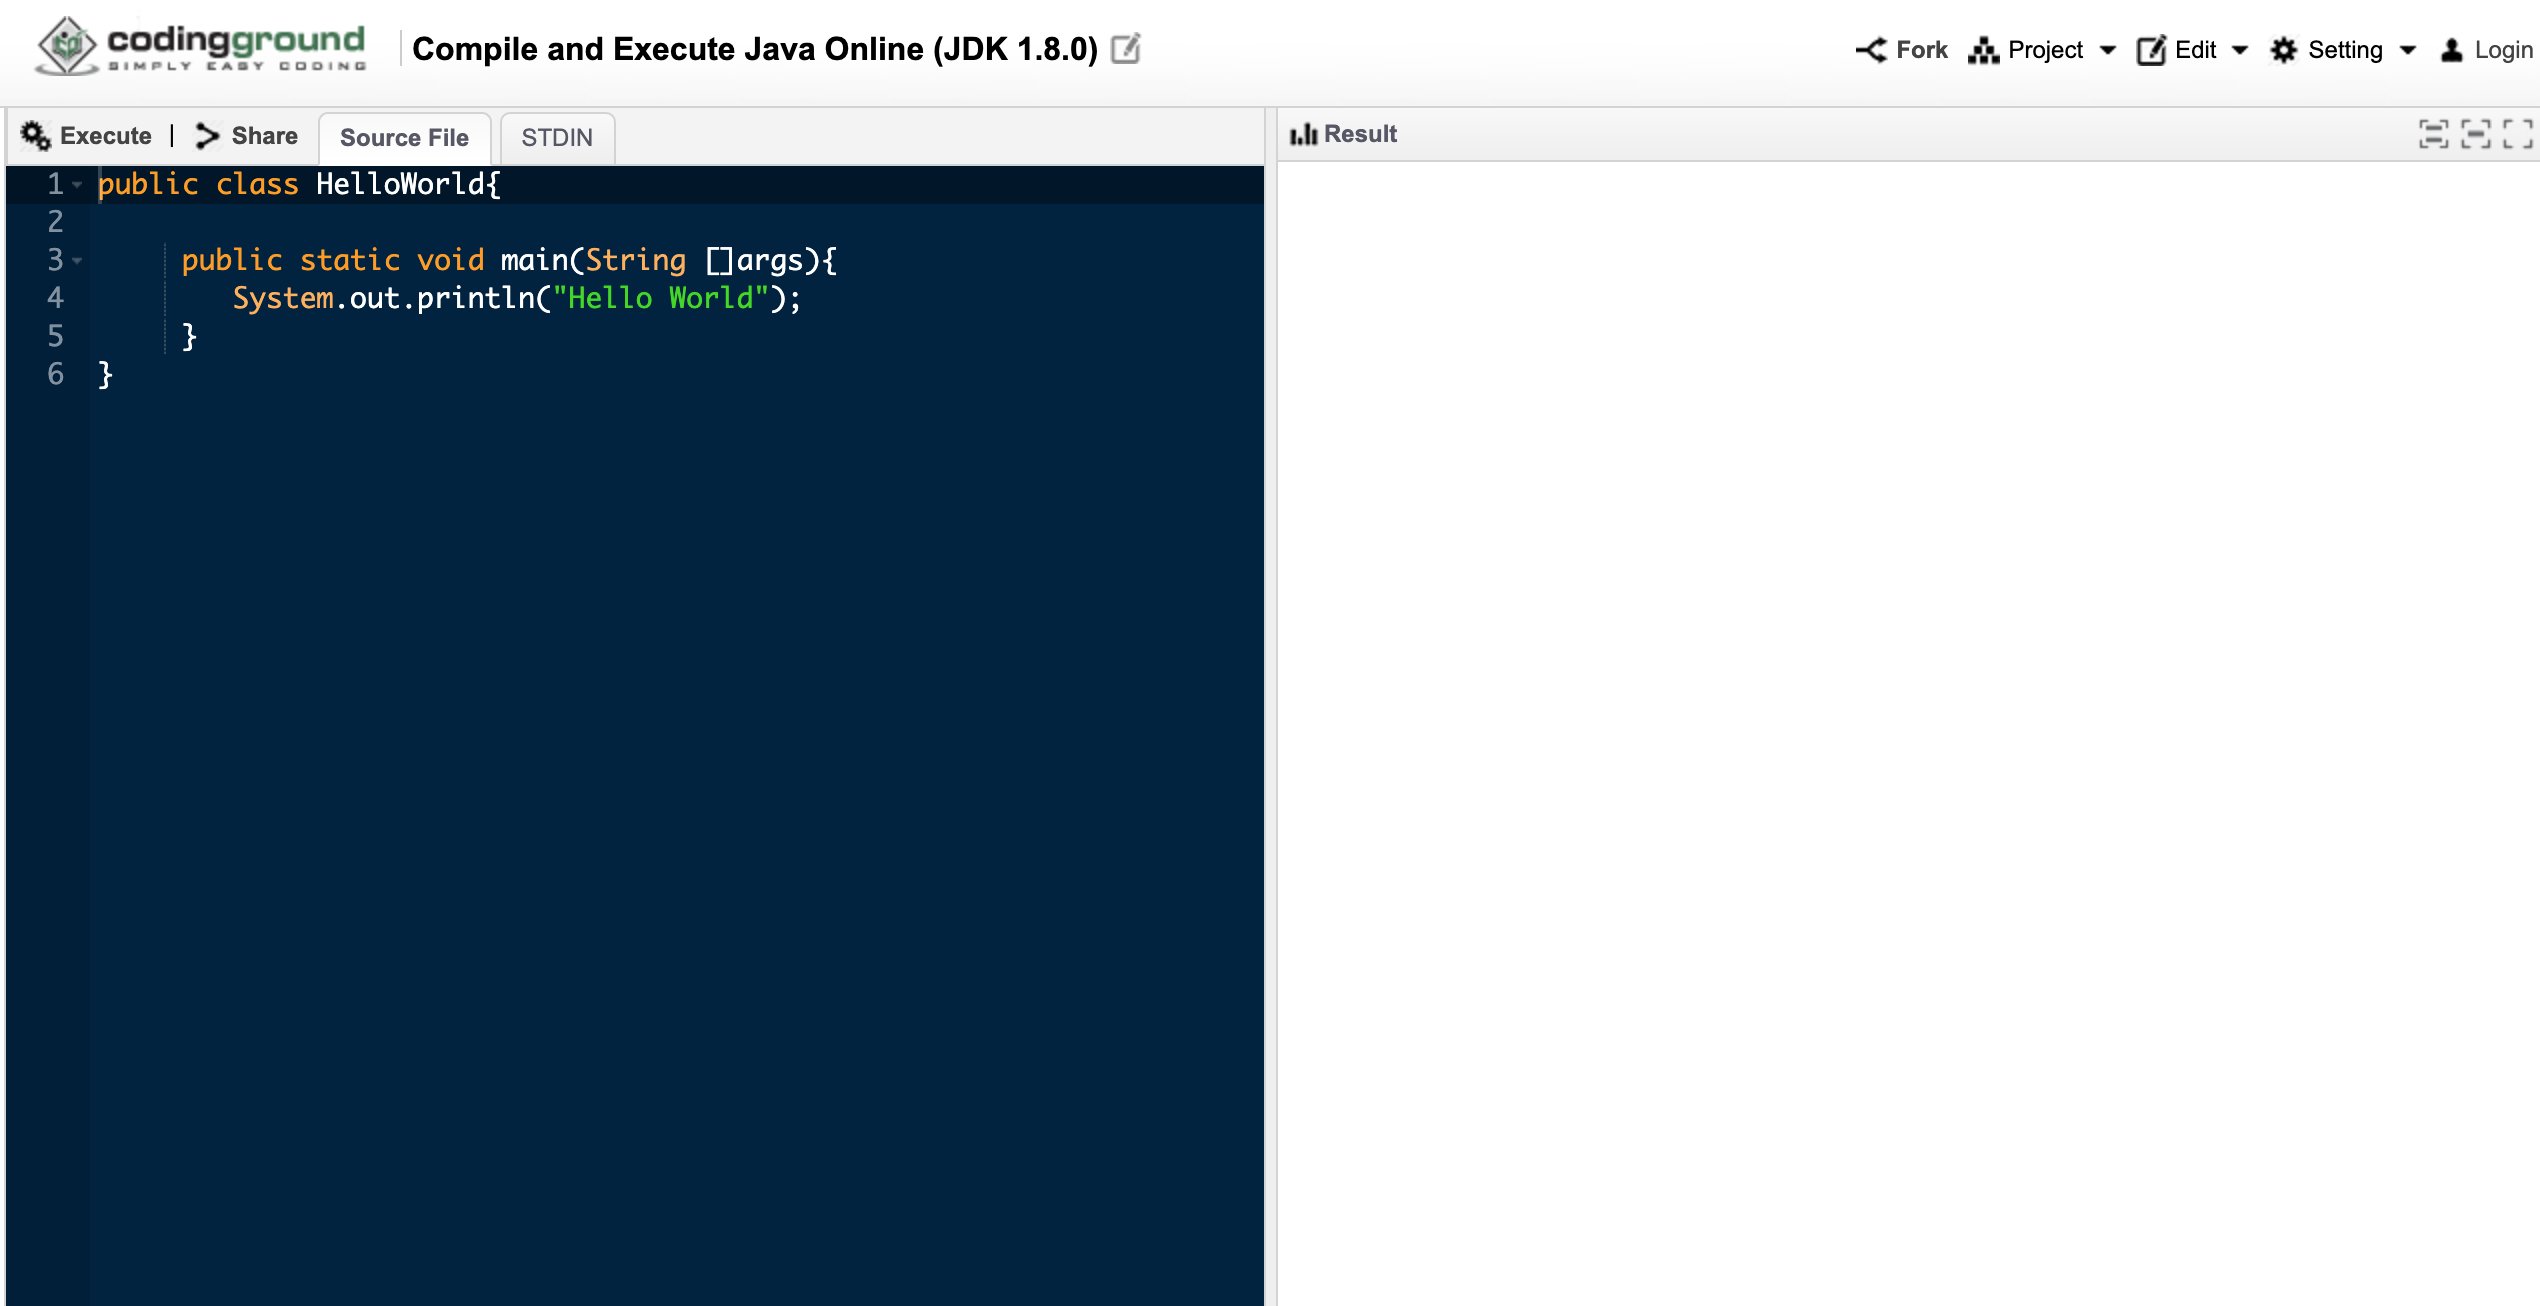
\includegraphics[scale=0.3]{java.png}
\end{center}
Java does not have REPL, hence there is no need to implement console input.
A slightly different has been taken by Haskell mode for emacs. 
\begin{center}
     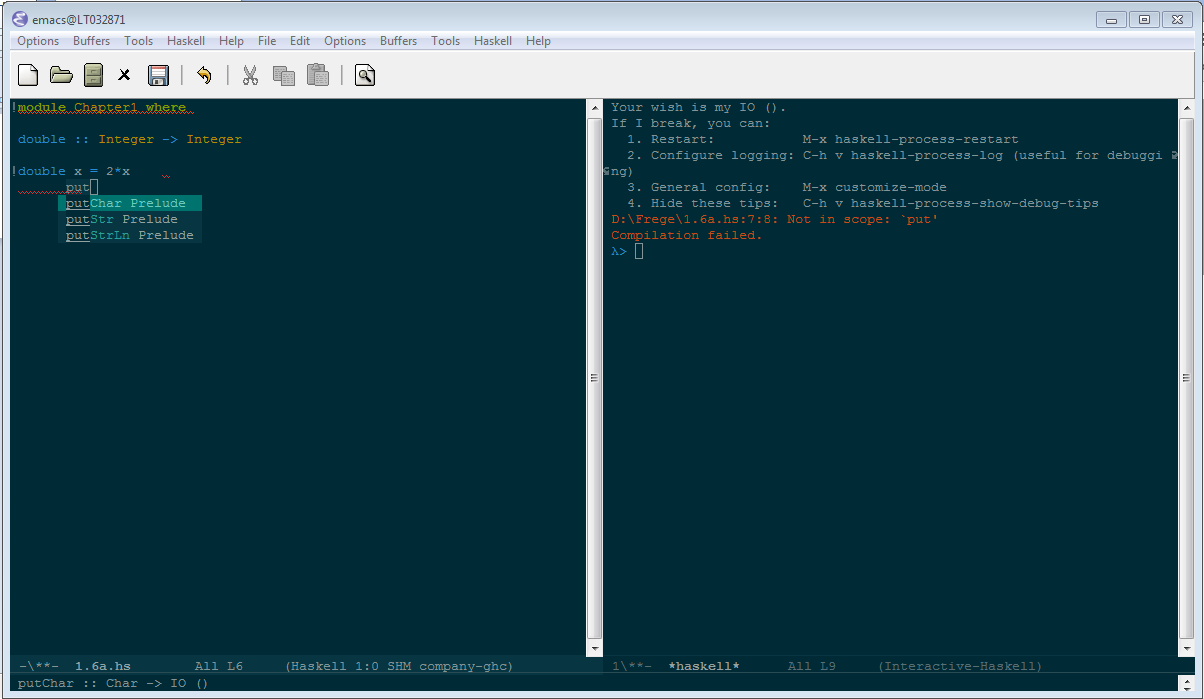
\includegraphics[scale=0.45]{haskell.png}
\end{center}
Here it is indeed possible to evaluate smaller snippets of code in the right window, while the left one is solely dedicated to editing local files that can be saved persistently. This is the approach that we settled for in our online playground for Solomonoff. 
\begin{center}
     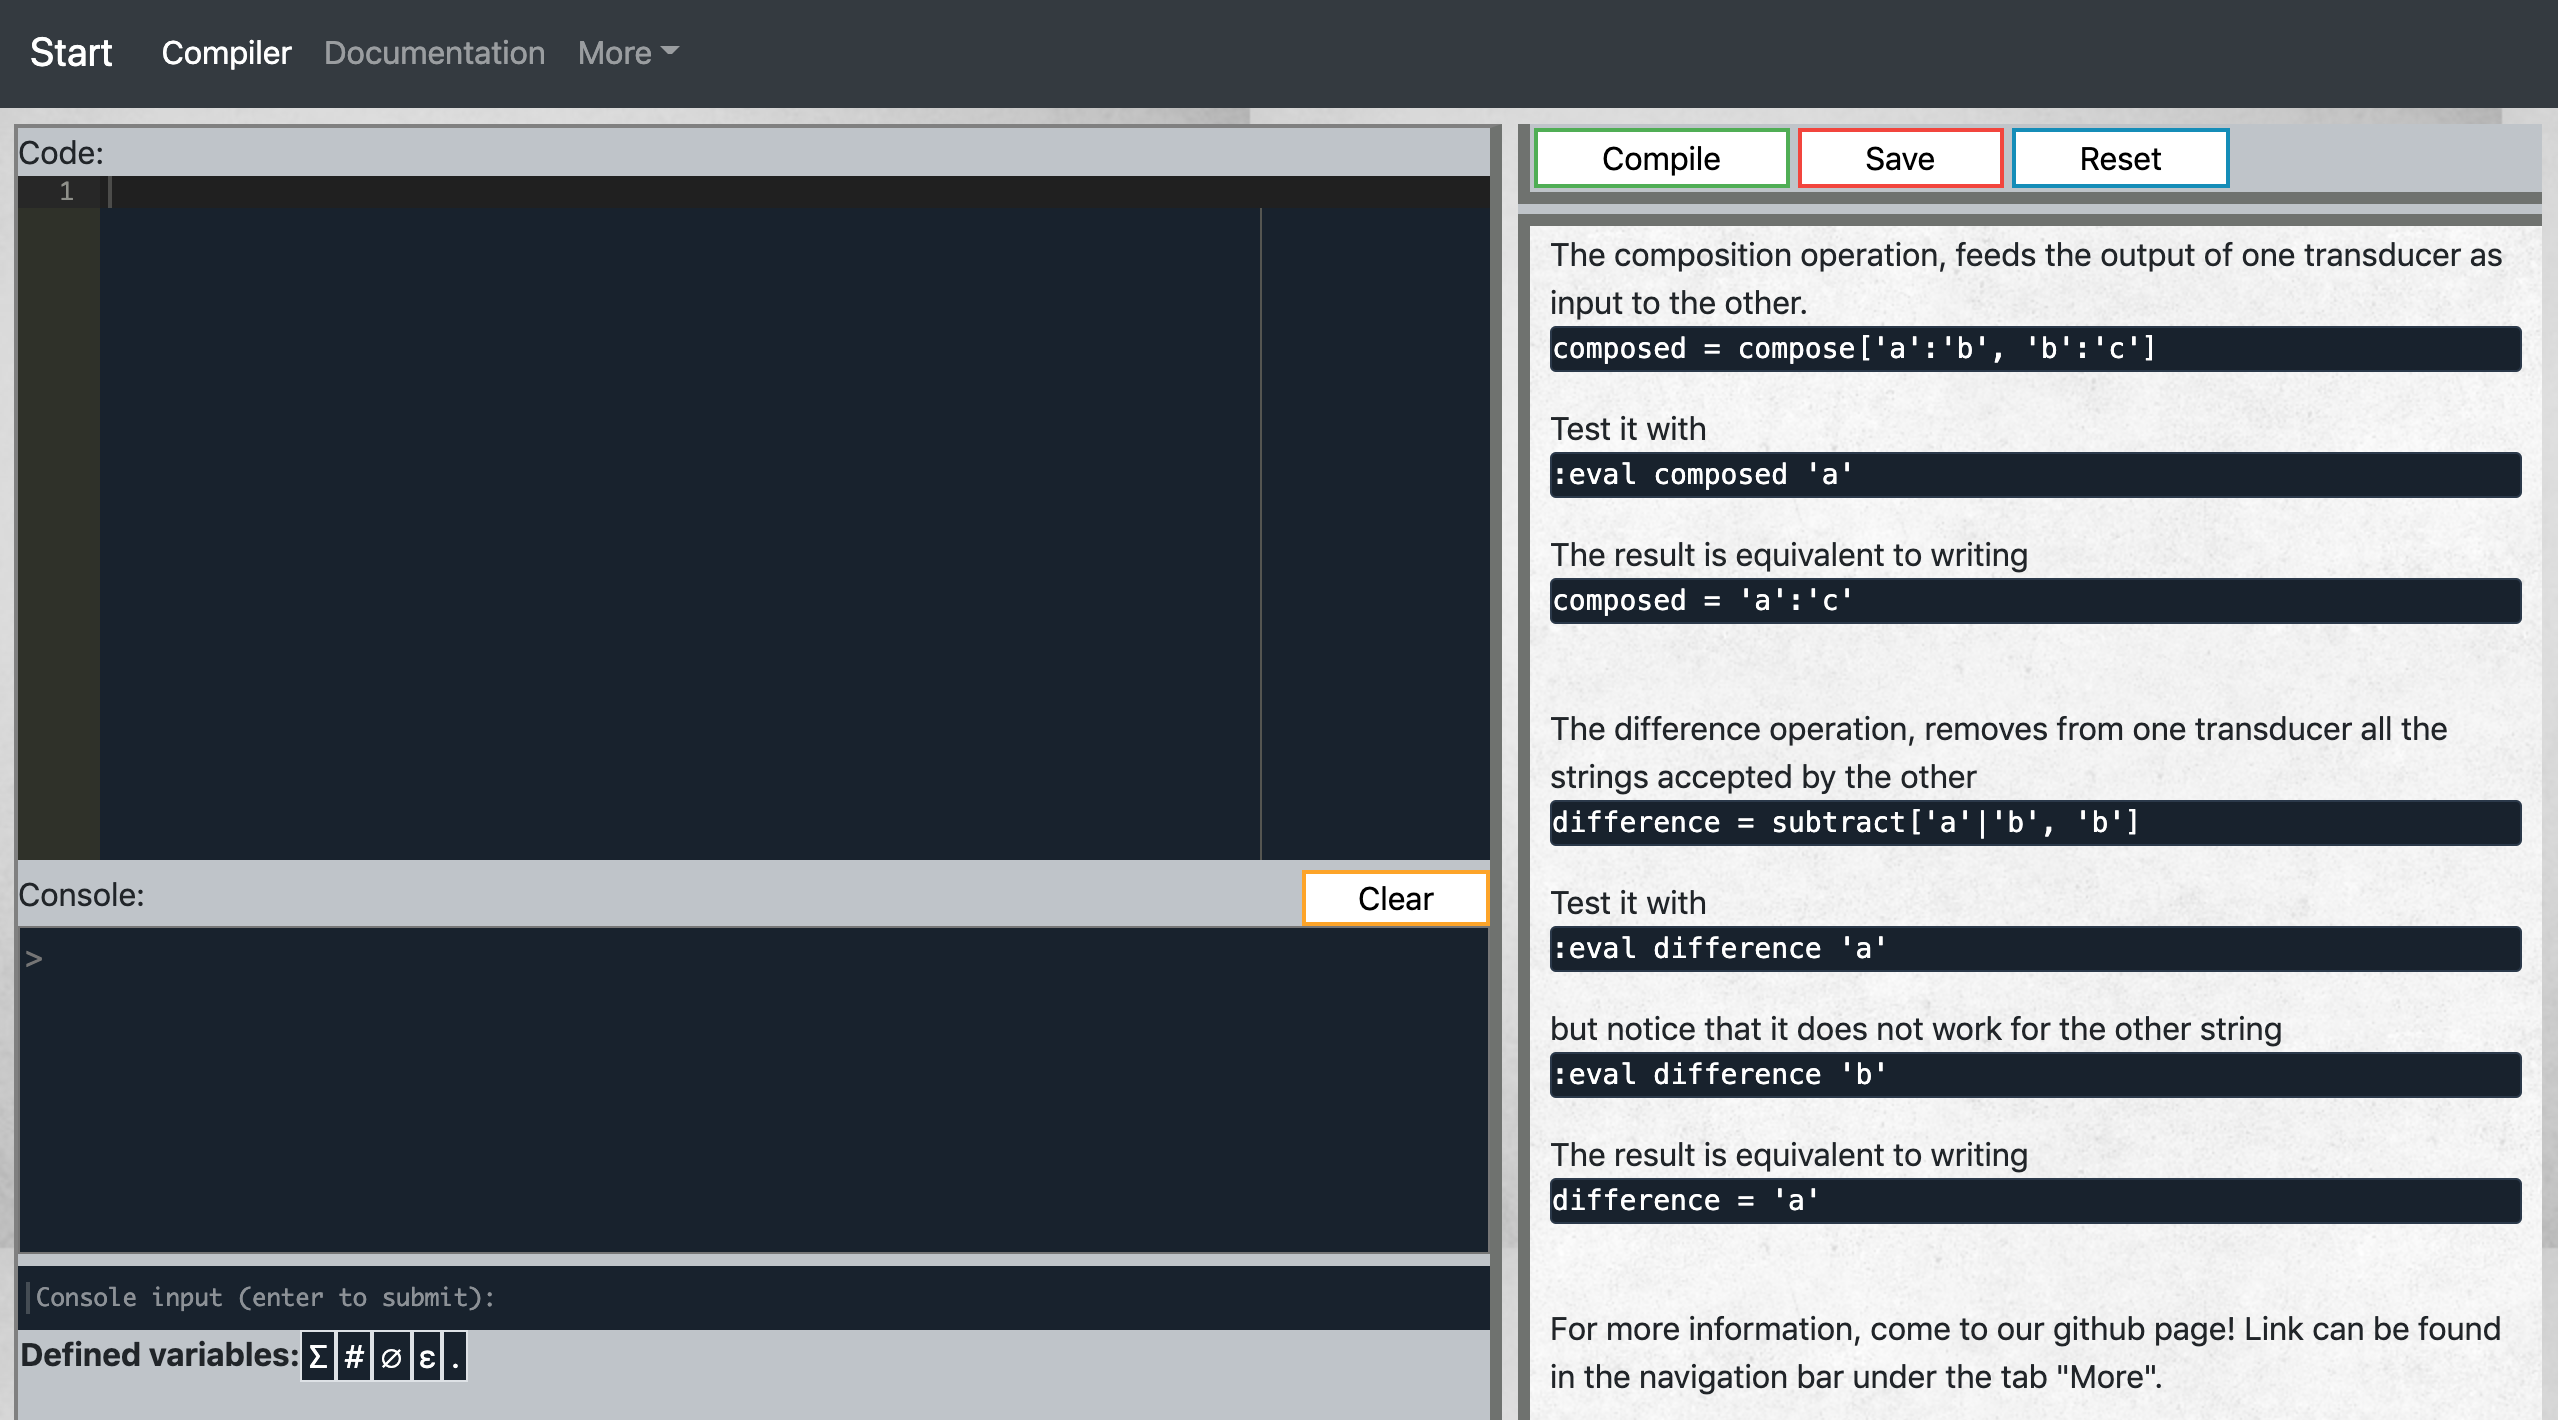
\includegraphics[scale=0.3]{web8.png}
\end{center}
Before reaching such final version we have experimented with another approach that seemed more natural for regular expressions. Here is an example of a similar website that evaluates UNIX regexes.
\begin{center}
     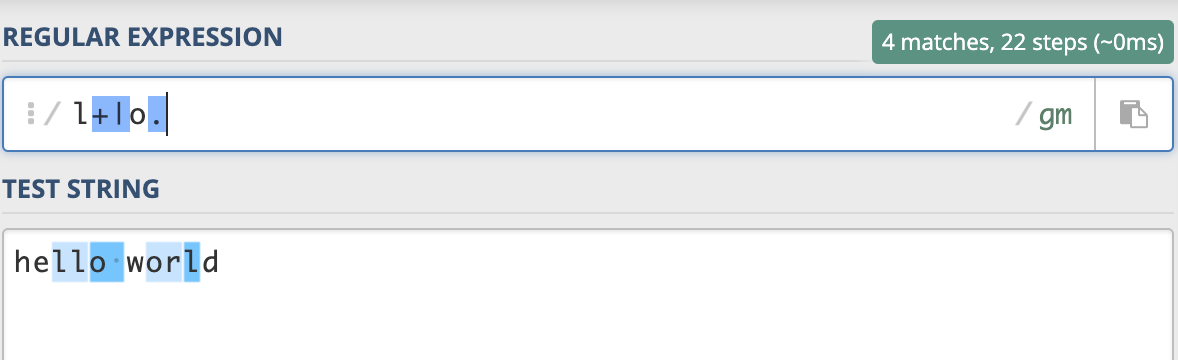
\includegraphics[scale=0.65]{regex.png}
\end{center}
Initially we tried to mimic such approach with some modifications. Solomonoff is much more complex than UNIX regexes. It allows variables, functions, comments and the overall code could consist of multiple lines. Hence a dedicated multiline editor window was required like in case of Java or Haskell.
\begin{center}
     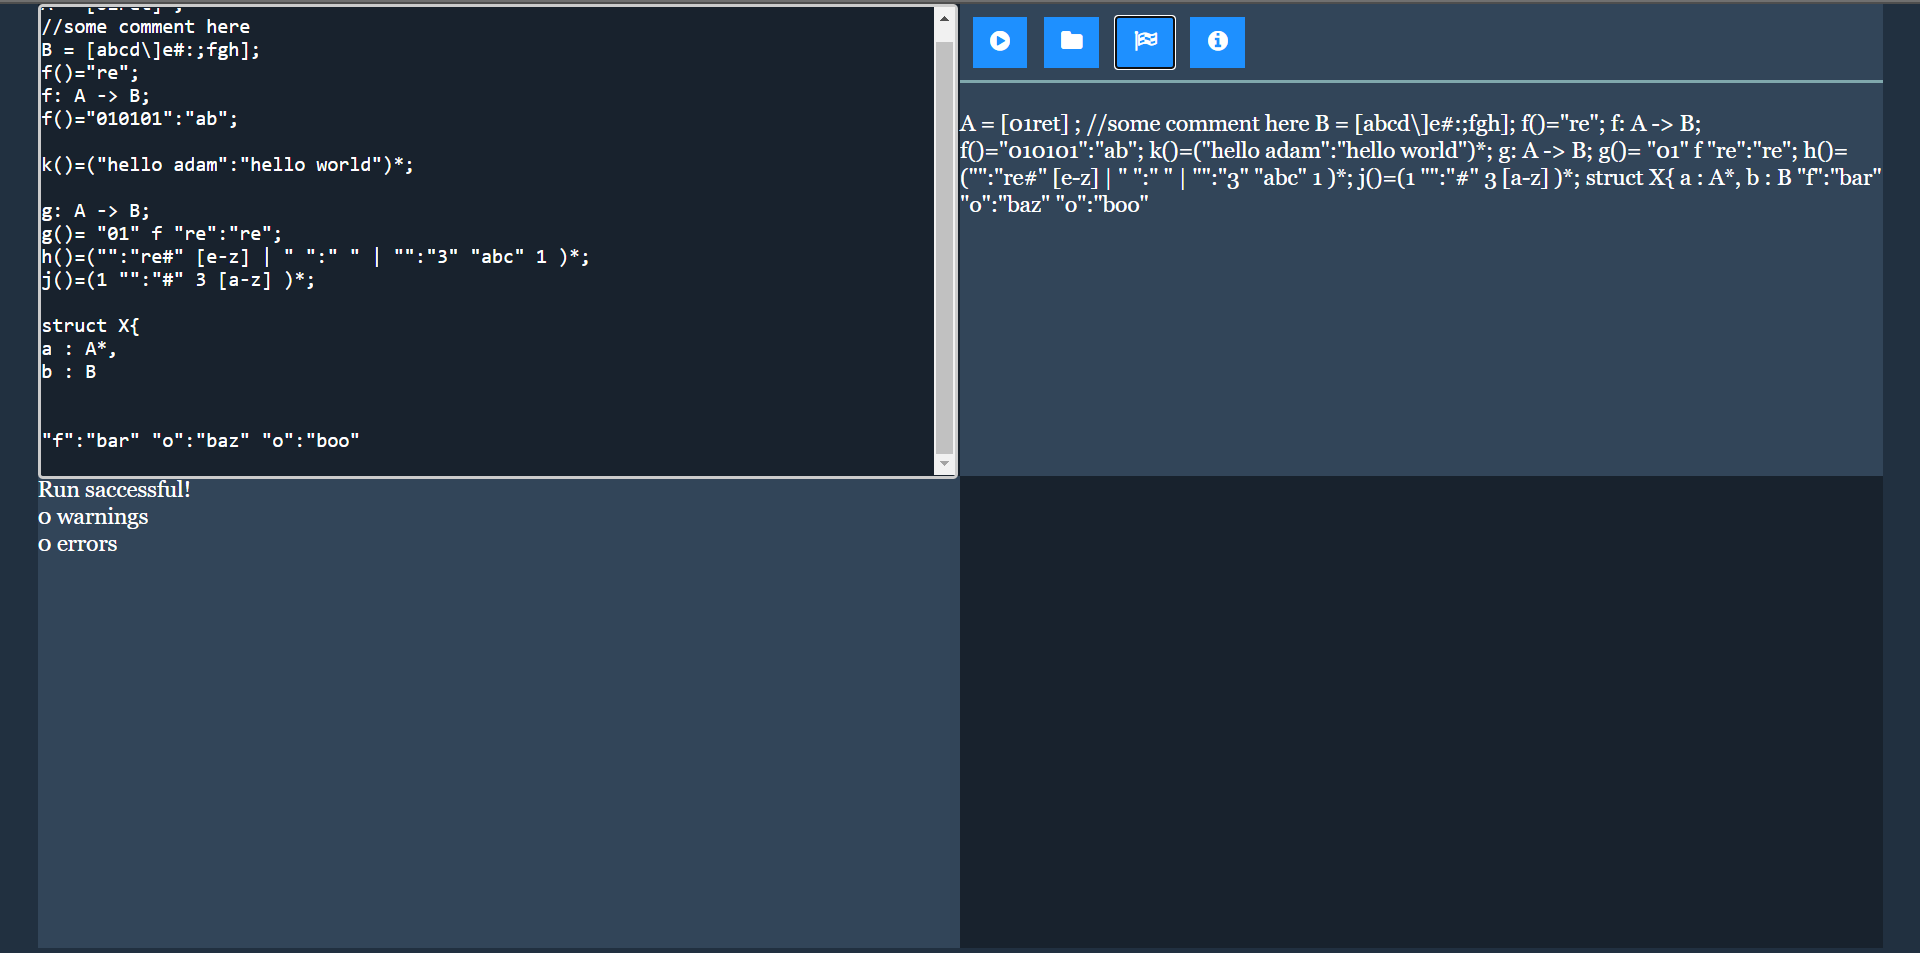
\includegraphics[scale=0.2]{web3.png}
\end{center}
The upper left window was dedicated to code. The lower left was meant to hold the test input string and the upper right would show the resulting transducer output. Such an approach seemed perfect at the beginning, when Solomonoff was still in early development. Over time, the language became increasingly complex. Several features were added that allowed for visualizing graphs of automata, sampling their languages, testing their formal properties and querying more complex information about them. The interface couldn't keep up with the full range of possibilities offered by he compiler. Hence, we decided to scrap the idea with two input-output windows and tried to emulate console-like REPL instead. The first version looked as follows
\begin{center}
     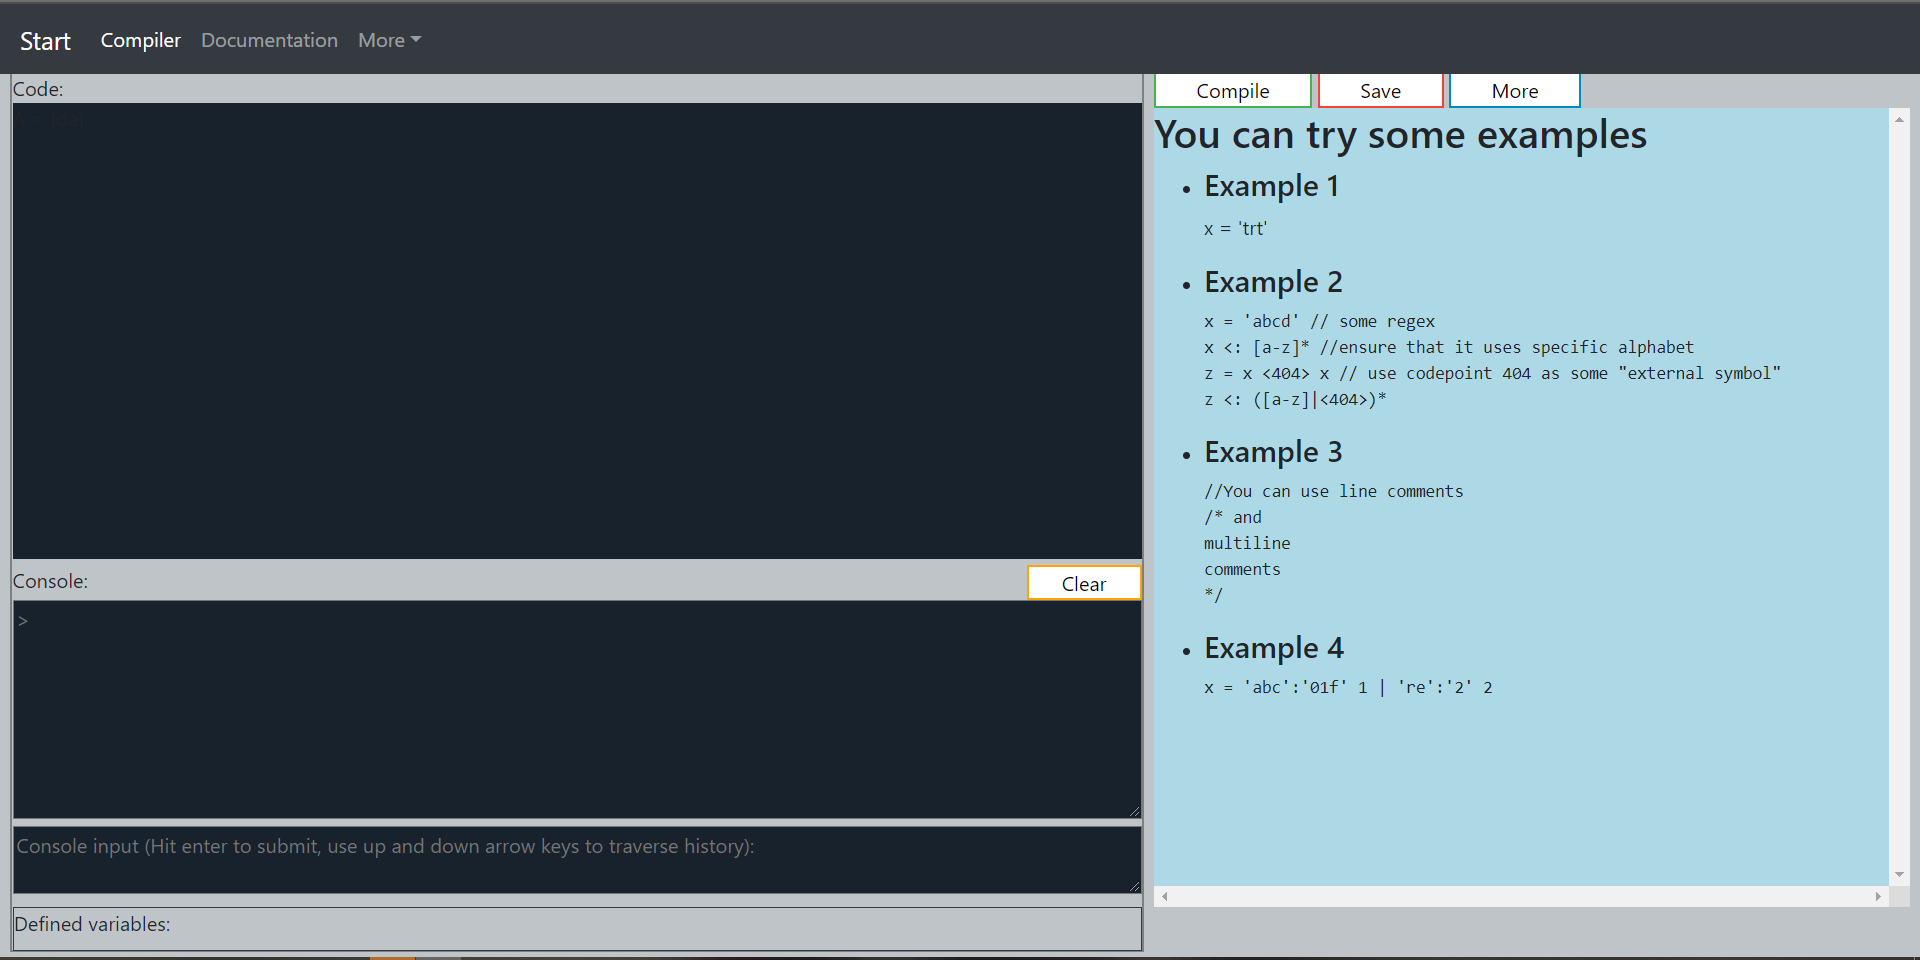
\includegraphics[scale=0.2]{web6.png}
\end{center}
It was at this point when we first tried to add a window for documentation. A great source of inspiration was the Alt-Ergo online playground. It comes with many helpful examples, which can be automatically copied to the editor upon clicking on them.
\begin{center}
     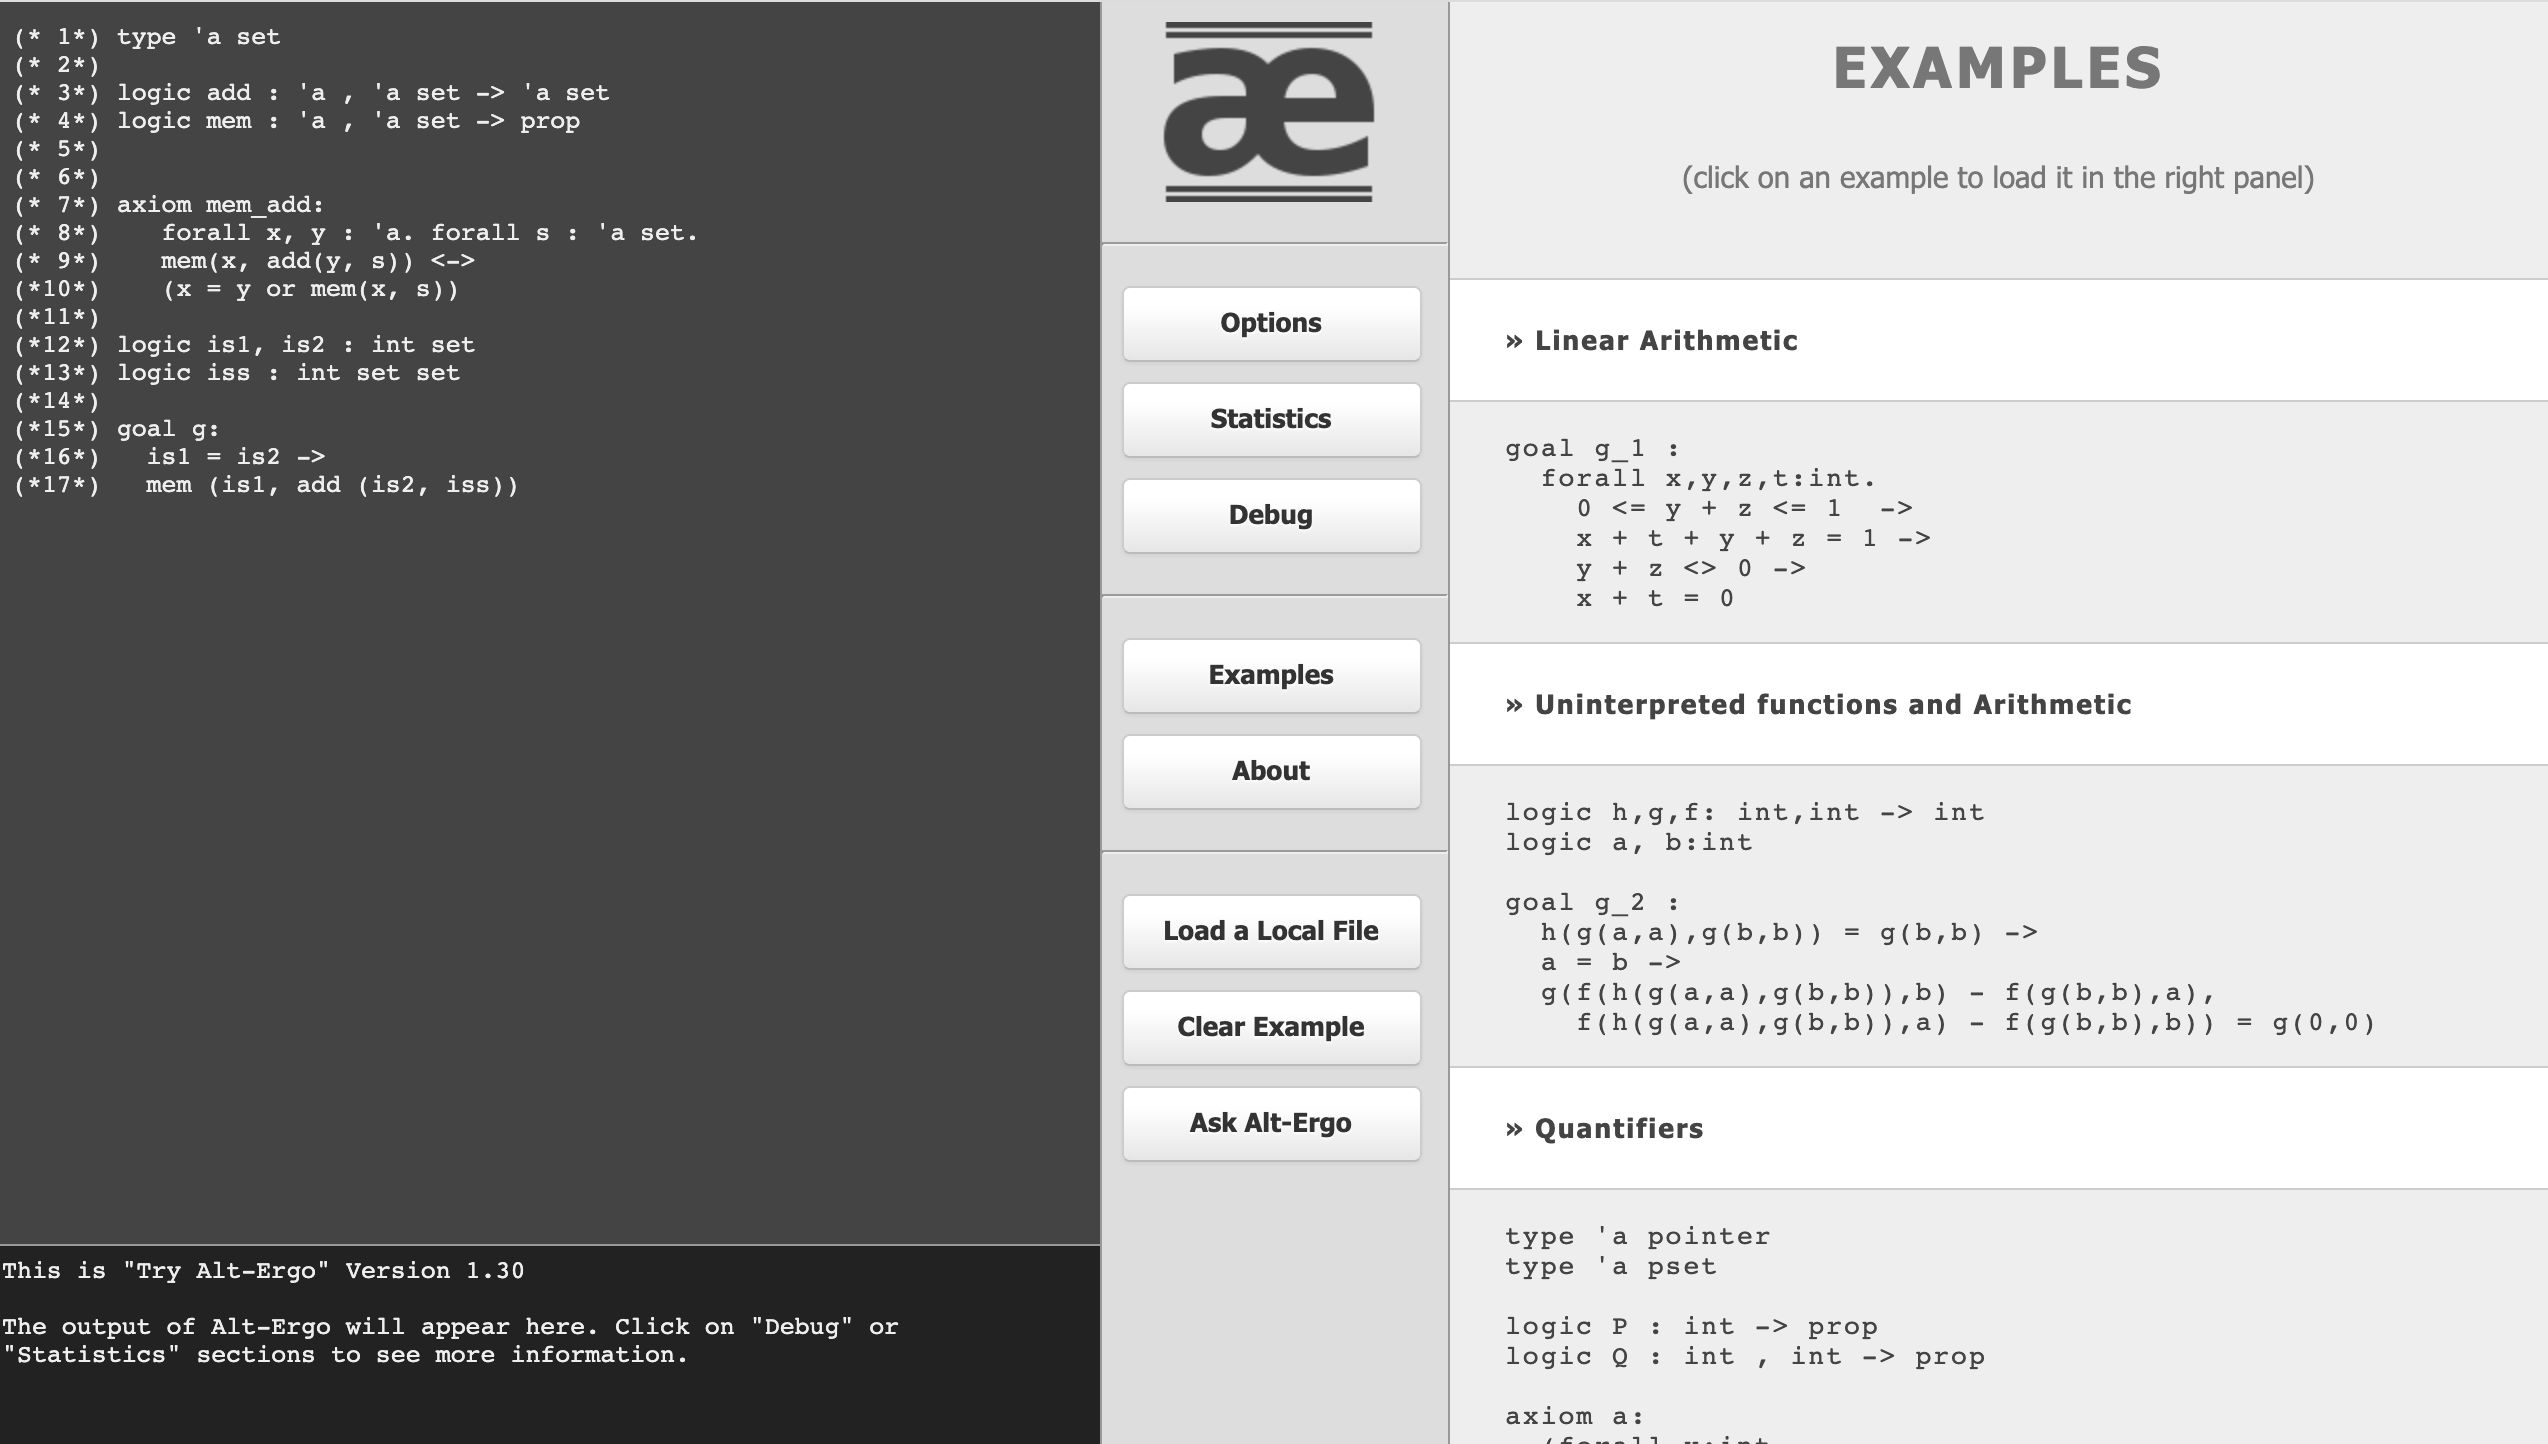
\includegraphics[scale=0.3]{alt-ergo.png}
\end{center}
Later we extended this idea to a full tutorial with explanations, rather than a simple list of copyable examples. 

\subsection{Ace editor}

At the same time as the layout of page evolved, we also actively developed the editor itself. While initially we used a simple HTML textarea element, we soon replaced it with the Ace editor. It allowed for integrating many additional features such as syntax highlighting, auto-suggestions, code snippets and marking errors. The core component of working with Ace was the necessity of developing our own syntax highlighting. All the previously mentioned come out-of-the box for existing languages, like JavaScript, C and Python. The matters get much more complicated, when one attempts to define their custom language. Ace documentation for syntax developers tends to be rather sparse. 

There exists a common framework followed by most syntax highlighters. Their configuration consists of two main components - the highlighting rules and the styling rules. The former consist of a set of regular expressions. Any region matched by a certain expression is marked with a list of styles. Then each style decides about the colour. Many existing text editors come with their own syntax highlighter and the required configurations may differ, albeit each format could be automatically converted into any other. 

By using the Iro editor, developer can develop only a single set of rules and then have them automatically converted to any other syntax highlighter. This includes support for Ace, SublimeText, TextMate and Atom. Most of the other editors, like Intellij, Eclipse, Notepad++ etc. use one of the above standards. 

The general format of Iro is as follows
\begin{lstlisting}

styles [] {
     
     .comment : style {
          color                 = #688557
          italic                = true
          ace_scope             = comment
          textmate_scope        = comment
          pygments_scope        = Comment
     }
 
}

main : context {
     
     : pattern {
          regex          \= (//.*)
          styles []       = .comment;
     }
 
}
\end{lstlisting}
each pattern matches some fragment of code and assigns a style to it. Then the style defines colour and scope. The scope is later used as a hint for various other tools that rely on syntax recognition. The colours themselves are also a mere hint. The end user might use an editor that supports various colour palettes. In particular many editors come with optional dark and light theme. Depending on user's choice, our colouring might be overriden. Hence the assigned scope is more important than the colour hint.

Most of the language grammars are context-free and cannot be recognized with a simple regular expression. Hence syntax highlighters allow for using stacks. A good example of this are the block comments. The regular expressions that apply outside of comments should not apply inside them. Iro allows developer to manipulate the stack using push and pop command.
\begin{lstlisting}
: inline_push {
     regex          \= (/\*)
     styles []       = .comment;
     default_style   = .comment
     : pop {
          regex       \= (\*/)
          styles []    = .comment;
     }
}
\end{lstlisting}
Solomonoff's syntax highlighter uses stack to correctly recognize comments and string literals enclosed in quotes and angle brackets. The rest of syntax highlighter is fairly simple and only matches key characters, such as equal signs, brackets, Kleene stars and union vertical pipes as well as variable identifiers.

After the syntax highlighter was developed, Iro automatically generated necessary Ace files. All those configurations are written JavaScript. In order to make them work, it's necessary to clone Ace's repository and compile the custom syntax along with the rest of sources. The compiled project needs to be hosted on website along with remaining JavaScript files. The Ace editor can be initialized using the following lines
\begin{lstlisting}
var editor = ace.edit("editor");
editor.session.setMode("ace/mode/mealy");
\end{lstlisting}
where \texttt{mealy} is the name of our custom syntax.
The editor has been styled using monokai theme
\begin{lstlisting}
editor.setTheme("ace/theme/monokai");
\end{lstlisting}
because its dark palette of colours gives the website a sharp and modern look. The dark theme is preferred by most users and is very popular nowadays. Moreover it's more relaxing to look at and doesn't irritate the eye. This point is especially important, because Solomonoff is targetted at tech-oriented audiences, so there is a good chance that our users will spend many hours looking at the editor. 

Solomonoff comes with several built-in functions. To make the interface more intuitive and ergonomic the editor needs to provide auto-suggestions with the full range available functions. Below is a list presenting some of the more important options.
\begin{lstlisting}
editor.setOptions({
     enableBasicAutocompletion: [{
          getCompletions: (editor, session, pos,
           prefix, callback) => {
               callback(null, [{
                    name: 'subtract[',
                    value: 'subtract[]',
                    score: 1,
                    meta: 'difference of two languages'
               },
               {
                    name: 'rpni!(',
                    value: 'rpni!()',
                    score: 1,
                    meta: 'RPNI inference algorithm'
               },
               {
                    name: 'rpni_mealy!(',
                    value: 'rpni_mealy!()',
                    score: 1,
                    meta: 'RPNI for Mealy machiens'
               },
               {
                    name: 'ostia!(',
                    value: 'ostia!()',
                    score: 1,
                    meta: 'OSTIA inference for transducers'
               },
               {
                    name: 'compose[',
                    value: 'compose[]',
                    score: 1,
                    meta: 'transducer composition'
               },
               {
                    name: 'inverse[',
                    value: 'inverse[]',
                    score: 1,
                    meta: 'transducer inversion'
               }
               ]);
          },
     }],
     enableSnippets: true,
     enableLiveAutocompletion: true
});
\end{lstlisting}
The \texttt{value} field is the text that autocompletion will produce when selected. The \texttt{meta} argument provides a short explanation that will be shown to the user. We decided to set \texttt{enableLiveAutocompletion} so that the dropdown box with all available functions will automatically show up as soon as the user starts typing. Some less experienced users might not be aware that the suggestions can be triggered manually by pressing \texttt{CTRL+SPACE}. The downside is that in some contexts the autosuggestion will pop up  despite not being necessary. This could irritate some users. Perhaps the best approach would be to make the auto-suggestions configurable. A user could set the editor properties according to their own liking. The only problem was that adding user customizations would increase the complexity of final product. Our goal was not to create a fully functioning IDE. The website is meant to work only as a showcase. Hence the final decision was to make the website as friendly to the newcomers as possible even at the cost of making the experienced users less comfortable. The general consensus was that users that like our product will quickly download the compiler locally and use it in conjunction with their own editor of choice. 

Initially, the Ace  was only used in the main editor window. The REPL console would be made of two text areas, one serving as editable input line and the other for console output, which was permanently set as non-editable. By design, the REPL commands could only be used in console and placing them in the main editor would only result in syntax errors. For instance
\begin{lstlisting}
:eval f 'input'
\end{lstlisting}
would only work in REPL, despite not being a valid Solomonoff code per se. As auto-suggestions were added, it became apparent that showing  REPL commands tin main editor would be very misleading
\begin{lstlisting}
editor.setOptions({
     enableBasicAutocompletion: [{
          getCompletions: (editor, session, pos,
          prefix, callback) => {
               callback(null, [
          ... 
               {
                    name: ':eval',
                    value: ':eval',
                    score: 1,
                    meta: 'evaluate transducer'
               }
          ...
               ]);
          },
     }],
     enableSnippets: true,
     enableLiveAutocompletion: true
});
\end{lstlisting}
On the other hand, not showing any hints related to REPL commands would seems like major shortcoming of the online playground. To address this issue it was later decided tha the REPL input line should also use Ace. As a result the website ended up with two instances of Ace editor. Both very similar to each other. The only difference being that auto-suggestions in REPL input would also display REPL commands, whereas the main code editor would not.

Using Ace in REPL input also happened to solve another problem. Every REPL command would have their own format of argument. For example the \texttt{:eval} would take transducer name and then some input string. The visualization only needs transducer name
\begin{lstlisting}
:vis f
\end{lstlisting}
 The most unintuitive is the random sample command which has two possible formats
 \begin{lstlisting}
:rand_sample f of_size 10
 \end{lstlisting}
and
 \begin{lstlisting}
:rand_sample f of_length 10
\end{lstlisting}
The former generates 10 random member strings, whereas the latter generates all member strings up to length of 10.
The \texttt{of\_size} and \texttt{of\_length} argument decides, which fo the two modes of generation to use. The initial idea to address this issue was to add user help displayed by the \texttt{:?} command.
\begin{lstlisting}
> :?
:vis [ID]
    Shows graph diagram of automaton
:rand_sample [ID] [of_size/of_length] [NUM]
    Generates random sample of input:output pairs produced 
    by ths transducer
:ls
    Lists all currently defined transducers
:clear
    Clears REPL console
:run [ID] [STRING]
    Runs pipeline for the given input
:unset [ID]
    Deletes a variable
:is_det [ID]
    Tests whether transducer is deterministic
:eval [ID] [STRING]
    Evaluates transducer on requested input
...
\end{lstlisting}
User could the consult this cheat sheet to determine format of arguments for each command. Such a solution was simple but it certainly didn't make for the most ergonomic user interface. With Ace it became possible to use code snippets instead.
Below are a few examples.
\begin{lstlisting}
getCompletions: (editor, session, pos, prefix, callback) => {
     callback(null, [
     {
          name: ':eval',
          value: ':eval',
          snippet: ':eval ${1:transducer_name} \'${2:input_string}\'',
          score: 1,
          meta: 'evaluate transducer'
     },
     {
          name: ':rand_sample of_size',
          value: ':rand_sample',
          snippet: ':rand_sample ${1:transducer_name} of_size ${2:number}',
          score: 1,
          meta: 'randomly generate sample'
     },
     {
          name: ':rand_sample of_length',
          value: ':rand_sample',
          snippet: ':rand_sample ${1:transducer_name} of_length ${2:number}',
          score: 1,
          meta: 'randomly generate sample'
     },
     ]);
}
\end{lstlisting}
The structure of arguments for each command was intuitively encoded in form
of blanks that need to be filled in each snippet. Each blank is specified using the \texttt{\$\{\}} braces.



\end{document}
